\documentclass{article}

% NOTES:
% This is a bad naming 
% - TODO: comment to indicate things to do
% - REF: comment to indicate a possible source to be cited
% - TODOREF: non-comment, indicates a future \cref{} for a missing figure/section/table/etc

% see readme
\def\OPTIONConf{1}%
\usepackage{joshuadunfield}
\usepackage{llproof}
% !TEX root = hazelnut-popl17.tex

% Violet hotdogs; highlight color helps distinguish them
\newcommand{\llparenthesiscolor}{\textcolor{violet}{\llparenthesis}}
\newcommand{\rrparenthesiscolor}{\textcolor{violet}{\rrparenthesis}}

% HTyp and HExp
\newcommand{\hcomplete}[1]{#1~\mathsf{complete}}

% HTyp
\newcommand{\htau}{\dot{\tau}}
\newcommand{\tarr}[2]{\inparens{#1 \rightarrow #2}}
\newcommand{\tarrnp}[2]{#1 \rightarrow #2}
\newcommand{\tnum}{\mathtt{num}}
\newcommand{\tehole}{\llparenthesiscolor\rrparenthesiscolor}
\newcommand{\tsum}[2]{\inparens{{#1} + {#2}}}

\newcommand{\tcompat}[2]{#1 \sim #2}
\newcommand{\tincompat}[2]{#1 \nsim #2}

% HExp
\newcommand{\hexp}{\dot{e}}
\newcommand{\hlam}[2]{\inparens{\lambda #1.#2}}
\newcommand{\hap}[2]{#1(#2)}
\newcommand{\hapP}[2]{(#1)~(#2)} % Extra paren around function term
\newcommand{\hnum}[1]{\underline{#1}}
\newcommand{\hadd}[2]{\inparens{#1 + #2}}
\newcommand{\hehole}{\llparenthesiscolor\rrparenthesiscolor}
\newcommand{\hhole}[1]{\llparenthesiscolor#1\rrparenthesiscolor}
\newcommand{\hindet}[1]{\lceil#1\rceil}
\newcommand{\hinj}[2]{\mathtt{inj}_{#1}({#2})}
\newcommand{\hcase}[5]{\mathtt{case}({#1},{#2}.{#3},{#4}.{#5})}

\newcommand{\hGamma}{\dot{\Gamma}}
\newcommand{\domof}[1]{\text{dom}(#1)}
\newcommand{\hsyn}[3]{#1 \vdash #2 \Rightarrow #3}
\newcommand{\hana}[3]{#1 \vdash #2 \Leftarrow #3}

% ZTyp and ZExp
\newcommand{\zlsel}[1]{{\bowtie}{#1}}
\newcommand{\zrsel}[1]{{#1}{\bowtie}}
\newcommand{\zwsel}[1]{
  \setlength{\fboxsep}{0pt}
  \colorbox{green!10!white!100}{
    \ensuremath{{{\textcolor{Green}{{\hspace{-2px}\triangleright}}}}{#1}{\textcolor{Green}{\triangleleft{\vphantom{\tehole}}}}}}
}

\newcommand{\removeSel}[1]{#1^{\diamond}}

% ZTyp
\newcommand{\ztau}{\hat{\tau}}

% ZExp
\newcommand{\zexp}{\hat{e}}

% Direction
\newcommand{\dParent}{\mathtt{parent}}
\newcommand{\dChildn}[1]{\mathtt{child}~\mathtt{{#1}}}
\newcommand{\dChildnm}[1]{\mathtt{child}~{#1}}

% Action
\newcommand{\aMove}[1]{\mathtt{move}~#1}
	\newcommand{\zrightmost}[1]{\mathsf{rightmost}(#1)}
	\newcommand{\zleftmost}[1]{\mathsf{leftmost}(#1)}
\newcommand{\aSelect}[1]{\mathtt{sel}~#1}
\newcommand{\aDel}{\mathtt{del}}
\newcommand{\aReplace}[1]{\mathtt{replace}~#1}
\newcommand{\aConstruct}[1]{\mathtt{construct}~#1}
\newcommand{\aConstructx}[1]{#1}
\newcommand{\aFinish}{\mathtt{finish}}

\newcommand{\performAna}[5]{#1 \vdash #2 \xlongrightarrow{#4} #5 \Leftarrow #3}
\newcommand{\performAnaI}[5]{#1 \vdash #2 \xlongrightarrow{#4}\hspace{-3px}{}^{*}~ #5 \Leftarrow #3}
\newcommand{\performSyn}[6]{#1 \vdash #2 \Rightarrow #3 \xlongrightarrow{#4} #5 \Rightarrow #6}
\newcommand{\performSynI}[6]{#1 \vdash #2 \Rightarrow #3 \xlongrightarrow{#4}\hspace{-3px}{}^{*}~ #5 \Rightarrow #6}
\newcommand{\performTyp}[3]{#1 \xlongrightarrow{#2} #3}
\newcommand{\performTypI}[3]{#1 \xlongrightarrow{#2}\hspace{-3px}{}^{*}~#3}

\newcommand{\performMove}[3]{#1 \xlongrightarrow{#2} #3}
\newcommand{\performDel}[2]{#1 \xlongrightarrow{\aDel} #2}

% Form
\newcommand{\farr}{\mathtt{arrow}}
\newcommand{\fnum}{\mathtt{num}}
\newcommand{\fsum}{\mathtt{sum}}

\newcommand{\fasc}{\mathtt{asc}}
\newcommand{\fvar}[1]{\mathtt{var}~#1}
\newcommand{\flam}[1]{\mathtt{lam}~#1}
\newcommand{\fap}{\mathtt{ap}}
% \newcommand{\farg}{\mathtt{arg}}
\newcommand{\fnumlit}[1]{\mathtt{lit}~#1}
\newcommand{\fplus}{\mathtt{plus}}
\newcommand{\fhole}{\mathtt{hole}}
\newcommand{\fnehole}{\mathtt{nehole}}

\newcommand{\finj}[1]{\mathtt{inj}~#1}
\newcommand{\fcase}[2]{\mathtt{case}~#1~#2}

% Talk about formal rules in example
\newcommand{\refrule}[1]{\textrm{Rule~(#1)}}

\newcommand{\herase}[1]{\left|#1\right|_\textsf{erase}}

\newcommand{\arrmatch}[2]{#1 \blacktriangleright_{\rightarrow} #2}


\newcommand{\TABperformAna}[5]{#1 \vdash & #2                & \xlongrightarrow{#4} & #5 & \Leftarrow #3}
\newcommand{\TABperformSyn}[6]{#1 \vdash & #2 \Rightarrow #3 & \xlongrightarrow{#4} & #5 \Rightarrow #6}
\newcommand{\TABperformTyp}[3]{& #1 & \xlongrightarrow{#2} & #3}

\newcommand{\TABperformMove}[3]{#1 & \xlongrightarrow{#2} & #3}
\newcommand{\TABperformDel}[2]{#1 \xlongrightarrow{\aDel} #2}

\newcommand{\sumhasmatched}[2]{#1 \mathrel{\textcolor{black}{\blacktriangleright_{+}}} #2}

\newcommand{\subminsyn}[1]{\mathsf{submin}_{\Rightarrow}(#1)}
\newcommand{\subminana}[1]{\mathsf{submin}_{\Leftarrow}(#1)}


\newcommand{\inparens}[1]{{\color{gray}(}#1{\color{gray})}}

%% rule names for appendix
\newcommand{\rname}[1]{\textsc{#1}}
\newcommand{\gap}{\vspace{7pt}}

% for header page
\newcommand{\vs}{\vspace{20pt}}

% for header page
\newcommand{\pt}[1]{\MakeUppercase{
    \centering{}
    \large{}
    #1 \\
    \vs{}
  }}

% allow custom lexer for pygmentize
% https://github.com/gpoore/minted/issues/176#issuecomment-695344998
\usepackage{minted}
\usepackage{regexpatch}

\makeatletter
\newcommand{\minted@def@optcl@novalue}[2]{%
  \define@key{minted@opt@g}{#1}[]{%
    \minted@addto@optlistcl{\minted@optlistcl@g}{#2}%
    \@namedef{minted@opt@g:#1}{#2}}%
  \define@key{minted@opt@g@i}{#1}[]{%
    \minted@addto@optlistcl{\minted@optlistcl@g@i}{#2}%
    \@namedef{minted@opt@g@i:#1}{#2}}%
  \define@key{minted@opt@lang}{#1}[]{%
    \minted@addto@optlistcl@lang{minted@optlistcl@lang\minted@lang}{#2}%
    \@namedef{minted@opt@lang\minted@lang:#1}{#2}}%
  \define@key{minted@opt@lang@i}{#1}[]{%
    \minted@addto@optlistcl@lang{%
      minted@optlistcl@lang\minted@lang @i}{#2}%
    \@namedef{minted@opt@lang\minted@lang @i:#1}{#2}}%
  \define@key{minted@opt@cmd}{#1}[]{%
    \minted@addto@optlistcl{\minted@optlistcl@cmd}{#2}%
    \@namedef{minted@opt@cmd:#1}{#2}}%
}

% new minted option "custom" for adding command line option "-x"
\minted@def@optcl@novalue{custom}{-x}

% new minted option "formatter=<formatter>" for specifying pygments formatter
\minted@def@opt{formatter}

% apply "-f <formatter>"
\newcommand\minted@formatter{%
  \minted@get@opt{formatter}{latex}\space
}

% Note: may require fix to regexpatch:
% https://tex.stackexchange.com/questions/578518/regexpatchcmd-failing-with-latex2e-2020-10-01-patch-level-4-use-cs-replacemen#comment1469403_578518
\xpatchcmd*\minted@checkstyle
  {-f latex }
  {-f \minted@formatter}
  {}{\fail}
\xpatchcmd*\minted@pygmentize
  {-f latex }
  {-f \minted@formatter}
  {}{\fail}

  \makeatother
  % end custom lexer for pygmatize

% Need VerbatimEnvironment:
% https://tex.stackexchange.com/a/400115
\newenvironment{hminted}
{\VerbatimEnvironment
\begin{minted}[escapeinside=//,frame=single,custom]{../latex-includes/hazel_lexer.py:HazelLexer}}
{\end{minted}}

% hazel inline; don't really know what's going on here
% https://tex.stackexchange.com/a/181393
\newcommand{\hmintinlinet}{
  \mintinline[escapeinside=//,frame=single,custom]{../latex-includes/hazel_lexer.py:HazelLexer}
}
\newcommand{\hmintinline}[1]{\expandafter\hmintinlinet\expandafter{#1}}

% \newcommand{\ab}{expanded stuff}
% \newcommand{\pythoninline}{\mintinline[]{python}}

% hazel inputminted
\newcommand{\inputhminted}[1]{\inputminted[escapeinside=//,frame=single,custom]{../latex-includes/hazel_lexer.py:HazelLexer}{lstings/#1.hz}}

% ocaml inputminted
\newcommand{\inputominted}[1]{\inputminted[escapeinside=//,frame=single]{ocaml}{lstings/#1.ml}}


% extra math operators
% especially for math operators that are introduced in this paper, want to
% declare them here so they are easily changeable
\DeclareMathOperator{\fix}{fix}       % fixpoint
\newcommand{\env}{\sigma}             % environment
\newcommand{\pp}{\Uparrow}            % post-process
\newcommand{\pplc}{\pp_{[]}}          % post-process lambda conversion (substitution) operator
\newcommand{\pplco}{\pp_{[],1}}       % post-process lc part 1
\newcommand{\pplct}{\pp_{[],2}}       % post-process lc part 2
\newcommand{\ppn}{\pp_{i}}            % post-process hole closure numbering
\newcommand{\ppnd}{\pp_{i,d}}         % post-process hole closure numbering (results only)
\newcommand{\ppns}{\pp_{i,\env}}      % post-process hole closure numbering (sigmas only)
\newcommand{\pplcl}{PPI$_{[]}$}       % post-process lambda within evaluation boundary conversion label
\newcommand{\pplclo}{PPO$_{[]}$}      % post-process lambda outside evaluation boundary conversion label
\newcommand{\ppndl}{PP$_{i,d}$}       % post-process hole closure numbering label
\newcommand{\ppnsl}{PP$_{i,\env}$}     % post-process hole closure numbering label
\newcommand{\pth}{p}                  % path
\newcommand{\hci}{H}                  % hole instance/closure info
\DeclareMathOperator{\hid}{hid}       % hole instance id generator

% for use in Hazel listings
\newcommand{\rar}{$\rightarrow$}
\newcommand{\Rar}{$\Rightarrow$}
\newcommand{\lbd}{$\lambda$}
\newcommand{\heh}[1]{$\hehole^{#1}$}

% for missing references
\newcommand{\todo}[1]{\textbf{[TODO: #1]}}
\newcommand{\todoref}[1]{\textbf{[TODO: need reference(s): #1]}}

%%% Local Variables:
%%% mode: latex
%%% TeX-master: "../thesis/main"
%%% End:


\usepackage{amsmath}
\usepackage{amssymb}
\usepackage{stmaryrd}
\usepackage{hyperref}
\usepackage{geometry}
\usepackage{setspace}
\usepackage{cleveref}
\usepackage{mdframed}
\usepackage[utf8]{inputenc}

% code listings
\usepackage{minted}

% https://tex.stackexchange.com/a/35547
\usepackage{etoolbox}
\AtBeginEnvironment{minted}{\singlespacing}

% % https://tex.stackexchange.com/a/55088
% \makeatletter{}
% \renewcommand\tableofcontents{%
%   \@starttoc{toc}%
% }
% \renewcommand\listoffigures{%
%   \@starttoc{lof}%
% }
\makeatother{}

% https://tex.stackexchange.com/a/132647
\usepackage{etoolbox}
\patchcmd{\thebibliography}{\section*{\refname}}{}{}{}

\begin{document}

\doublespacing
\pagenumbering{roman}

% title and signature pages
\thispagestyle{empty}

{
  \centering
  \large

  \pt{
    The Cooper Union for the Advancement of Science and Art \\
    Albert Nerken School of Engineering
  }
  
  \vfill{}
  
  {
    {
      \huge
      Optimization by memoization of evaluation tasks \\
      in the Hazel structured programming environment \\
    }
    \vs{}
    by Jonathan Lam \\
  }

  \vfill{}

  {
    A thesis submitted in partial fulfillment of the requirements for the degree of \\
    Master of Engineering \\
  }

  \vfill{}

  {
    Professor Fred L. Fontaine, Advisor \\
    Professor Robert Marano, Co-advisor \\
    % TODO: Can I add Prof. Omar on the title page too?
  }


  \vfill{}
  {
    Performed in collaboration with the \\
    Future of Programming Lab at the University of Michigan \\
  }
}

%%% Local Variables:
%%% mode: latex
%%% TeX-master: "main"
%%% End:

\thispagestyle{empty}

{
  \pt{
    The Cooper Union for the Advancement of Science and Art \\
    Albert Nerken School of Engineering
  }
  
  \noindent{} This thesis was prepared under the direction of the Candidate's Thesis Advisor and has received approval. It was submitted to the Dean of the School of Engineering and the full Faculty, and was approved as partial fulfillment of the requirements for the degree of Master of Engineering.
}

\vfill{}

\begin{singlespace}
  \raggedleft{}
  \rule{0.5\textwidth}{1pt} \\
  \makebox[0.5\textwidth][r]{
    Barry L. Shoop, Ph.D., P.E. \hfill Date
  } \\
\end{singlespace}

\vfill{}

\begin{singlespace}
  \raggedright{}
  \rule{0.5\textwidth}{1pt} \\
  \makebox[0.5\textwidth][l]{
    Fred L. Fontaine, Ph.D. \hfill Date
  } \\
\end{singlespace}

\vfill{}
\vfill{}

%%% Local Variables:
%%% mode: latex
%%% TeX-master: "main"
%%% End:

\pt{Acknowledgments}

TODO

% Family, aunt/uncles/everyone i've lived with
% 10B
% Victor and Derek
% Advisor, UMich ppl

%%% Local Variables:
%%% mode: latex
%%% TeX-master: "main"
%%% End:

\pt{Abstract}

\noindent{}Hazel is a live programming environment with typed holes that serves as a reference implementation of Hazelnut Live dynamic semantics and the Hazelnut static semantics, both of which tackle the ``gap problem.'' This work attempts to further develop the Hazel evaluation model by implementing the environment model of evaluation (rather than the current substitution model) and memoizing several evaluation-related operations to improve performance. Additionally, we provide an implementation-level description and a reference implementation of the fill-and-resume (FAR) performance optimization proposed in Hazelnut Live. We produce a metatheory and reference implementation of the proposed changes. We also benchmark the our implementation against the existing Hazel implementation and show that the results match the expectation, although there is room for future improvement with further development of FAR. Finally, we discuss some useful theoretical generalizations that result from this work and how we hope this work informs future development on Hazel.

%%% Local Variables:
%%% mode: latex
%%% TeX-master: "main"
%%% End:


% toc and lof
\pt{Table of contents}
\tableofcontents{}
\clearpage{}
\pt{List of figures}
\listoffigures{}

% list of nomenclature/terminology/notation
\pt{List of notations}
% \FloatBarrier{}

% nomencl package is too confusing, just use manual tables

\newcommand{\colwidths}{p{4cm}p{10cm}}

\singlespacing

\begin{table}[H]
  \centering
  \begin{tabular}{\colwidths}
    \hline\hline
    $e$ & (External) expression \\
    $\tau$ & Type \\
    $\Gamma$ & Typing context \\
    $\Delta$ & Hole context \\
    $\Gamma\vdash e:\tau$ & Type judgment \\
    $\Gamma\vdash e\Rightarrow\tau$ & Synthetic type judgment \\
    $\Gamma\vdash e\Leftarrow\tau$ & Analytic type judgment \\
    $[e'/x]e$ & Substitution of $e'$ for $x$ in $e$ \\
    \hline\hline
  \end{tabular}
  \caption{Common notation for the $\lambda$-calculus}
  \label{tab:symb_general}
\end{table}

\begin{table}[H]
  \centering
  \begin{tabular}{\colwidths}
    \hline\hline
    \ulc & Untyped $\lambda$-calculus \\
    \stlc & Simply-typed $\lambda$-calculus \\
    \gtlc & Gradually-typed $\lambda$-calculus \\
    $\Lambda_{\rightarrow}^{\tehole}$ & $\lambda$-calculus with typed holes \\
    \hline\hline
  \end{tabular}
  \caption{The $\lambda$-calculi}
  \label{tab:symb_general}
\end{table}

\begin{table}[H]
  \centering
  \begin{tabular}{\colwidths}
    \hline\hline
    $\gtlch$ & Unknown type \\
    $\tau\sim\tau'$ & Type consistency \\
    $\arrmatch{\tau}{\tau_1\to\tau_2}$ & Matched arrow judgment \\
    $\Gamma\vdash e\leadsto d:\tau$ & Elaboration judgment \\
    $d\langle\tau\Rightarrow\tau'\rangle$ & Cast expression \\
    \hline\hline
  \end{tabular}
  \caption{The gradually-typed $\lambda$-calculus}
  \label{tab:symb_general}
\end{table}

\begin{table}[H]
  \centering
  \begin{tabular}{\colwidths}
    \hline\hline
    $d$ & Internal expression \\
    $\lambda x:\tau.d$ & $\lambda$-abstraction \\
    $\fix f:\tau.d$ & Fixpoint form \\
    $\env$ & Environment \\
    $x,f$ & Variable name \\
    $u$ & Hole number \\
    $i$ & Hole instance or closure number \\
    $\hehole^{u:i}$ & Empty hole expression \\
    $\hhole{d}^{u:i}$ & Non-empty hole expression \\
    $[\env]d$ & Generalized closure \\
    \hline\hline
  \end{tabular}
  \caption{Hazel internal language}
  \label{tab:symb_hazel_dhexp}
\end{table}

\begin{table}[H]
  \centering
  \begin{tabular}{\colwidths}
    \hline\hline
    $d\textsf{ value}$ & Value \\
    $d\textsf{ final}$ & Final \\
    $\env\vdash d\Downarrow d'$ & Evaluation \\
    \hline\hline
  \end{tabular}
  \caption{Hazel evaluation judgments}
  \label{tab:symb_hazel_dhexp}
\end{table}

\begin{table}[H]
  \centering
  \begin{tabular}{\colwidths}
    \hline\hline
    $\hci$ & Hole instance/closure information \\
    $\hid$ & Hole instance/closure id generation function \\
    $\pth$ & Hole closure parent \\
    $d\pp d'$ & Postprocessing \\
    $d\pplc d'$ & Postprocessing ($\lambda$-conversion) \\
    $\hci,\pth\vdash d\ppn d'\dashv\hci'$ & Postprocessing (hole closure numbering) \\
    \hline\hline
  \end{tabular}
  \caption{Hazel postprocessing judgments}
  \label{tab:symb_hazel_dhexp}
\end{table}

\begin{table}[H]
  \centering
  \begin{tabular}{\colwidths}
    \hline\hline
    $\nodiff{d_1}{d_2}$ & No diff (empty diff) between $d_1$ and $d_2$ \\
    $\nfdiff{d_1}{d_2}$ & Non-fill diff from $d_1$ to $d_2$ \\
    $\fdiff{d_1}{d_2}{u}{d}$ & Fill diff from $d_1$ to $d_2$ with fill parameters $u$ and $d$ \\
    $\sdiff{d_1}{d_2}{u}{d}$ & Some (non-empty) diff from $d_1$ to $d_2$ \\
    $\adiff{d_1}{d_2}{u}{d}$ & Any (possibly empty) diff from $d_1$ to $d_2$ \\
    $d_1\sim d_2$ & Expression form equality \\
    \hline\hline
  \end{tabular}
  \caption{Fill-and-resume structural diff algorithm}
  \label{tab:symb_far-diff}
\end{table}

\begin{table}[H]
  \centering
  \begin{tabular}{\colwidths}
    \hline\hline
    $\far{u}{d}{d'}=d''$ & Fill-and-resume operation on an expression \\
    $\far{u}{d}{\env}=\env'$ & Fill-and-resume operation on an environment \\
    $\llbracket\env\rrbracket d$ & Closure with re-eval flag set \\
    $\hhole{d}_i$ & Expression $d$ filled in hole with hole closure number $i$ \\
    $\fenv$ & Fill memoization context\\
    $\env,\fenv\vdash d\Downarrow d'\dashv\fenv'$ & Fill-memoized evaluation \\
    \hline\hline
  \end{tabular}
  \caption{Fill-and-resume pre-processing and evaluation}
  \label{tab:symb_far-eval}
\end{table}

\doublespacing

%%% Local Variables:
%%% mode: latex
%%% TeX-master: "main"
%%% End:


% end front matter
\pagenumbering{arabic}
\clearpage{}

\chapter{Introduction}
\label{sec:introduction}

\section{Problem statement}
\label{sec:prob_stmt}

\begin{figure}
  \centering
  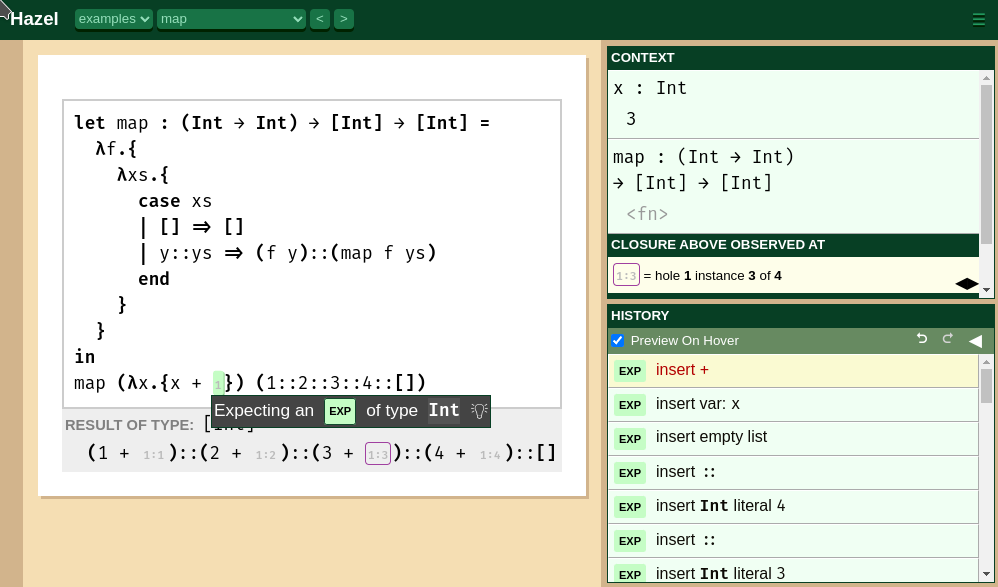
\includegraphics[width=4in]{img/hazel_ui.png}
  \caption[Screenshot of the Hazel live programming environment.]{A screenshot of the Hazel live programming environment. Screenshot taken of the dev branch demo on 02/06/2022 \cite{HazelDemo2022}.}
  \label{fig:screenshot-hazel-ui}
\end{figure}

Unstructured plaintext editing has remained the dominant mode of programming for decades, but makes it more difficult to implement editor services to aid the process. Structural editors, on the other hand, only allow valid edit states. Several structural editors, such as Scratch \cite{maloney2010scratch}, Lamdu \cite{lotem_chuchem}, and mbeddr \cite{voelter2012mbeddr}, have been proposed to improve the programming experience and introduce editor services, such as the elimination of syntax errors or graphical editing.

Hazel \cite{hazel_git} is an experimental structural language definition and implementation that aims to solve the ``gap problem'': spatial and temporal holes that temporarily prevent code from being able to be compiled or evaluated. The structural editor is defined by a bidirectional edit calculus Hazelnut \cite{conf/popl/Hazelnut17}, which governs the structural editor and the static semantics (typing rules) of the language. The dynamic semantics (evaluation semantics) are described in Hazelnut Live \cite{conf/popl/HazelnutLive19}.

Hazel is a relatively new research effort by the University of Michigan's Future of Programming Lab (FPLab), with little effort placed on performance optimizations. This work attempts to achieve several enhancements to Hazelnut Live that will benefit the performance of evaluation and related tasks. Part of the work will be focused on transitioning the evaluation model from using substitution for variable bindings to using environments, with emphasis on evaluation of holes and postprocessing of the evaluation result to match the result from evaluation with substitution. The latter parts of this work will use the environment model of evaluation to improve the memoization of certain tasks specific to Hazel (such as hole closure numbering), and also implement the fill-and-resume performance enhancement described in \cite{conf/popl/HazelnutLive19}. The novelty of this work lies in the optimization capacity in the unique design of the Hazel language as a live programming editor with expression holes.

\section{The contribution of this work}
\label{sec:contribution}

This thesis presents several algorithms designed for Hazel's evaluation. These algorithms are provided using the big-step inference semantics notation introduced in \cref{sec:semantics-notation}.

Firstly, we provide the evaluation semantics of the Hazel language using the environment model. We aim to keep the implementation pure, introduce uniquely-numbered environments (for later use in memoization), and describe the evaluation of holes (which are unique to Hazel). We introduce the concepts of generalized closures, and the evaluation boundary.

Secondly, we describe the postprocessing algorithm, which is mostly memoized by environments and has the two major functions. The first is to convert the result to the equivalent result if substitution was used. The second is to number hole closure instances.

Lastly, we develop the fill-and-resume process, as originally proposed (but not implemented) in \cite{conf/popl/HazelnutLive19}. We provide a possible implementation, including an algorithm to detect a valid fill operation and advice on memoizing the resumption operation.

The performance of this work is measured primarily in terms of empirical performance gains (via evaluation-step counting and benchmarking), and discussed with respect to the theoretical performance. Hazelnut \cite{conf/popl/Hazelnut17} and Hazelnut Live \cite{conf/popl/HazelnutLive19} mechanize proofs of their work using the Agda interactive proof checker. We do not provide mechanized proofs of our work; instead, we provide a series of core metatheorems describing invariants describing Hazel evaluation, and argue the correctness of these metatheorems by informal reasoning on the provided inference rules. A mechanized proof using Agda is deferred for future work.

\section{Structural overview}
\label{sec:structural_overview}

\Cref{sec:prog_lang_principles} provides a background on necessary topics in programming language (PL) theory and programming language implementations, in order to frame the understanding for the Hazel live programming environment. \Cref{sec:hazel} provides an overview of Hazel, in order to frame the work completed for this thesis project. \Crefrange{sec:env_model_evaluation}{sec:far_impl} describe the primary work completed for this project, as described in \Cref{sec:contribution}. \Cref{sec:evaluation} comprises an emprical performance assessment of the work. \Cref{sec:discussion} is a discussion of theoretical results. \Cref{sec:future_work} describes unfinished work and future research directions. \Cref{sec:concl} concludes with a summary of findings and future work. The Appendices contain extra inference rules and selected source code snippets.

%%% Local Variables:
%%% mode: latex
%%% TeX-master: "main"
%%% End:

\section{Programming language principles}
\label{sec:prog_lang_principles}

This chapter is intended to provide a primer to the theory of functional programming and programming languages, as relevant to this work on Hazel.

\subsection{Functional programming}
\label{sec:fp}

Functional programming \todoref{functional programming} is a programming paradigm that is highly involved with function application, function composition, and first-class functions. It is generally a subtype of, and often associated with, the declarative programming paradigm, which is concerned with expression-based computation, often without mutable state or side-effects. Declarative programming is often considered the complement of imperative programming, which may be characterized as programming with mutable state, side effects, or statements. Purely functional programming is a subset of functional programming that deals solely with pure functions; non-pure languages may allow varying degrees of mutable state but typically encourage the use of pure functions.

Functional languages are based on Alonzo Church's $\lambda$ calculus \todoref{lambda calculus} as its core evaluation and typing semantics, which provides a minimal foundation for computation. The syntax of functional programming languages is based off the $\lambda$ calculus. This, along with the lack of mutable state and side effects, allows functional programming to be easily mathematically modeled and reasoned about, making it particularly amenable to proofs about programming languages. This is as opposed to in imperative programming, in which the mutable ``memory cell'' interpretation of variables and side-effects complicates formalizations.

Hazel is one such (purely) functional programming languages. Other languages that are classified as functional include the ML family of languages, Haskell, Elm, and the LISP family of languages. Examples of imperative programming languages include C, C++, FORTRAN, Java, and Golang. A number of languages incorporate both functional and imperative styles, such as Javascript, Python, Scala, and Rust \todoref{all of these languages and their classifications}.

% TODO: show a simple example of programs in these paradigms

\subsubsection{The $\lambda$-calculus}
\label{sec:lambda-calculus}

\todo{this section is a mess at the moment; sorry}

The simplest form of the $\lambda$ calculus, the \textit{untyped $\lambda$ calculus}, comprises only three expression forms:
\begin{align}
  \label{eq:untyped-lambda-calculus}
  x\tag{Variable} \\
  \lambda x.e\tag{$\lambda$ abstraction} \\
  e_1\ e_2\tag{Function application}
\end{align}
where $e$, $e_1$, and $e_2$ are also expressions of one of these three forms. A $\lambda$ abstraction is also known as a $\lambda$ expression, $\lambda$ function, anonymous function, or simply function, and function application is also known as function invocation or $\beta$-reduction\footnote{A few notes for the imperative programmer: $\lambda$ functions only take a single parameter. A function of multiple parameters may be constructed as a series of recursive functions, each taking a single parameter -- a process known as \textit{currying}. Similarly, function application comprises two expressions, the first in \textit{function position} (which must evaluate to a $\lambda$ function), and the second in \textit{argument position}. Function application is traditionally (e.g., in the ML and Haskell families of programming languages, although LISP is an exception) denoted using the infix operator `` '' (space), which has the highest precedence of any infix operator; parentheses are only used to indicate order of operations and typically omitted when not necessary.}. The only reduction in the untyped $\lambda$ calculus is $\beta$-reduction, which is stated as follows.\[(\lambda x.e_1)\ e_2\to [e_1/x]e_2\] The notation $[x/y]z$ indicates substitution, and may be pronounced ``the substitution of $x$ for $y$ in $z$.'' According to computability theory, since the untyped $\lambda$ calculus supports general recursion (through the use of a fixpoint operator), it is Turing-complete.

While the untyped $\lambda$ calculus is Turing-complete and thus as expressive as any other Turing-complete programming language, this is far too tedious to be of any practical use. In this minimal foundation, we do not have base types such as integers or booleans\footnote{In the untyped $\lambda$ calculus, the only value type are $\lambda$ abstractions. Any other data type, such as the set of natural numbers or booleans, may be represented using $\lambda$ abstractions via \textit{Church encoding}.} or a typing system. The typical formulation of the \textit{simply-typed $\lambda$ calculus} extends the untyped $\lambda$ calculus with a (non-$\lambda$ abstraction) base type $b$ of type $B$, and a type $\tau\in $ TODO: working here; this is a mess

% TODO: describe these using syntax and semantics

% TODO: move syntax and semantics and notation to here

% TODO: describe typing rules

% TODO: for practical purposes, let and case expressions

% TODO: introduce gradually-typed lambda calculus

\subsubsection{Purity and statefulness}
\label{sec:purity}

\subsubsection{The ML family, Elm, and Hazel}
\label{sec:ml-fam}

% ADTs
% typing system

\subsection{Implementations for programming languages}
\label{sec:interpreters}

In order for a programming language to be practical, it must not only be defined as a set of syntax and semantics, but also have an \textit{implementation} to run programs in the language. Hazel is implemented as an interpreted language, whose runtime is transpiled to Javascript so that it may be run as a client-side web application in the browser.

It is important to note that the definition of a language (its syntax and semantics) are largely orthogonal to its implementation. In other words, a programming language does not dictate whether it requires a compiler or interpreter implementation, and languages sometimes have multiple implementations.

\subsubsection{Compiler vs. interpreter implementations}
\label{sec:comp-vs-interp}

There are two general classes of programming language implementations: \textit{interpreters} and \textit{compilers} \cite{aho86}. Both types of implementations share the function of taking a program as input, and should be able to produce the same result (assuming an equal and determinstic machine state, equal inputs, correct implementations, and no exceptional behavior due to differences in resource usage).

A compiler is a programming language implementation that converts the program to some low-level representation that is natively executable on the hardware architecture (e.g., x86-64 assembly for most modern personal computers, or the virtualized JVM architecture) before evaluation. This process typically comprises \textit{lexing} (breaking down into atomic tokens) the program text, \textit{parsing} the lexed tokens into a suitable \textit{intermediate representation} (IR) such as LLVM, performing optimization passes on the intermediate representation, and then generating the target bytecode (such as x86-64 assembly) \cite{aho86}. The bytecode outputted from the compilation process is used for evaluation. Compiled implementations tend to produce better runtime efficiency, since the compilation steps are performed separate of the evaluation, and because there is little to no runtime overhead.

An interpreter is a programming language implementation that does not compile down to native bytecode, and thus requires an interpreter or \textit{runtime}, which performs the evaluation. Interpreters still require lexing and parsing, and may have any number of optimization stages, but do not generate bytecode for the native machine, instead evaluating the program directly.

In certain contexts (especially in the ML spheres), the term \textit{elaboration} \cite{harper2000type} is used to the process of transforming the \textit{external language} (a well-formed, textual program) into the \textit{internal language} (IR). The interior language may include additional information not present in the external language, such as types generated by type inference or bidirectional typing.

The distinction between compiled and interpreted languages is not a very clear line: some implementations feature just-in-time (JIT) compilation that allow ``on-the-fly'' compilation (e.g., common implementations of the JVM and CLR \cite{sestoft2002runtime}), and some implementations may perform the lexing and parsing separately to generate a non-native bytecode representation to be later evaluated by a runtime. A general characterization of compiled vs. interpreted languages is the amount of runtime overhead required by the implementation.

Hazel is a purely interpreted language implementation, as optimizations for speed are not among its main concerns. However, performance is clearly one of the main concerns of this thesis project, but the gains will be algorithmic and use the nature of Hazel's structural editing and hole calculus to benefit performance, rather than changing the fundamental implementation. There is, however, a separate endeavor to write a compiled interpretation of Hazel \cite{hazelc}, which is outside the scope of this project.

\subsubsection{The substitution and environment models of evaluation}
\label{sec:sub-vs-eval}

% REF: https://cs.brown.edu/courses/cs173/2012/book/From_Substitution_to_Environments.html
% REF: https://www.cs.bham.ac.uk/research/projects/poplog/paradigms_lectures/lecture18.html
%   this introduces the issue with special forms like set! in a non-functional context

Evaluation in Hazel was originally performed using a \textit{substitution model of evaluation}, which is a theoretically simpler model. In this model, variables that are bound by some construct are substituted into the construct's body. For example, the variable(s) bound using a \mintinline{ocaml}|let|-expression pattern are substituted in the \mintinline{ocaml}|let|-expression's body, and the variable(s) bound during a function application are substituted into the function's body, and then the body is evaluated.

% TODO: show example of this

In this formulation, variables are ``given meaning'' via substitution; once evaluation reaches an expression, all variables in scope (in the typing context) will have been replaced by their value by some containing binding expression. In other words, variables are never evaluated directly; they are substituted by their values when bound, and their values are evaluated. The substitution model is useful for teaching purposes because it is simple and close to its mathematical definition: a variable can be thought of as an equivalent stand-in for its value.

However, for the purpose of computational efficiency, a model in which values are lazily expanded (``looked-up'') only when needed is more efficient. This is called the \textit{environment model of evaluation}, and generally is more efficient because the runtime does not need to perform an extra substitution pass over subexpressions and because untraversed (unevaluated) branches do not require substituting. Lastly, the runtime does not need to carry an expression-level IR of the language, due to the fact that the substitution model manipulates expressions, while evaluation does not. This means that the latter is more amenable for compilation, and is how compiled languages tend to be implemented: each frame of the theoretical stack frame is a de facto environment frame. While switching from the substitution to environment model is not an improvement in asymptotic efficency, these effects are useful especially for high-performance and compiled languages.

Note that the substitution model does not imply a lazy (i.e., normal-order, call-by-name, call-by-need) evaluation \cite{plotkin1975call} as in languages such as Haskell or Miranda, in which bound variables are (by default) not evaluated until their value is required. Laziness is conceptually tied to substitution, but the substitution model does not require laziness. Like most programming languages, Hazel only has strict (i.e., applicative-order, call-by-value) evaluation: the expressions bound to variables are evaluated at the time of binding.

% TODO: "Laziness is conceptually tied to substitution" -- but does it require substitution? Methinks so but not sure;
%   will find out more later due to this independent study

The implementation of evaluation with environments differs from that of evaluation with substitution primarily in that: an evaluation environment is required to look up bound variables as evaluation reaches them; binding constructs extend the evaluation environment rather than performing substitution; and $\lambda$ abstractions are bound with their evaluation environment at runtime to form (lexical) closures.

\subsection{Programming language semantics}
\label{sec:type-systems}

\subsubsection{Notation}
\label{sec:semantics-notation}

% little-step vs. big-step

\subsubsection{Static and dynamic semantics}
\label{sec:static-dynamic-semantics}

\subsubsection{Gradual typing}
\label{sec:gradual}

% \subsection{Approaches to programming interfaces}
% \label{sec:prog_intf}

% \subsubsection{Structure editors}
% \label{sec:structure_editors}

% \subsubsection{Graphical editors}
% \label{sec:graphical_editors}

% \subsubsection{Intentional, generative, and meta-programming}
% \label{sec:intentional_programming}

% \subsubsection{Applications to programming education}
% \label{sec:programming_education}

% \subsubsection{Drawbacks of non-textual editors}
% \label{sec:textual_benefits}

%%% Local Variables:
%%% mode: latex
%%% TeX-master: "main"
%%% End:

\chapter{An overview of the Hazel programming environment}
\label{sec:hazel}

Hazel is the reference implementation for the Hazelnut bidirectionally-typed action semantics and the Hazelnut Live dynamic semantics. It is intended to serve as a proof-of-concept of the semantics with static holes that attempt to mitigate the gap problem; however, the implementation is becoming increasingly practical with recent additions to the language. The reference implementation is an interpreter written in OCaml and transpiled to Javascript using the \mintinline{text}|js_of_ocaml| (JSOO) library \cite{vouillon2014bytecode} so that it may be run client-side in the browser. A screenshot of the reference implementation is shown in \Cref{fig:screenshot-hazel-ui} \cite{HazelDemo2022}. The source code may be found on GitHub \cite{Hazel2022}. Hazel may be characterized as a purely functional, statically-typed, bidirectionally-typed, strict-order evaluation, structured editor programming language.

\section{Motivation for Hazel}
\label{sec:hazel-motivation}

\subsection{The gap problem}
\label{sec:gap-problem}

Programming editor environments aim to provide feedback to a programmer in the form of editor services such as syntax highlighting or warnings using the LSP. Live programming environments aim to provide continuous static (static type error) and dynamic (run-time type error) feedback in real-time, allowing for rapid prototyping. However, over the course of the lifetime of a program, the program may enter many edit states when it is \textit{meaningless} (ill-formed or ill-typed).

Editor services can only assign static and dynamic meaning to programs that are statically well-typed and free of dynamic type errors. Some may deploy reduced ad hoc algorithms of meaningless edit states. This means that over the course of editing, the programmer experiences temporal gaps between moments of complete editor services. This is known as the \textit{gap problem} \cite{10.1145/2499370.2462170,conf/popl/HazelnutLive19}.

\subsection{An intuitive introduction to typed expression holes}
\label{sec:typed-holes}

Hazelnut and Hazelnut Live address the gap problem by defining a static and dynamic semantics, respectively, for a small functional programming language extended with typed holes. It is built on top of a \textit{structure editor}, which ensures that a program is always well-formed (syntactically correct) by disallowing invalid edit actions. The Hazelnut action semantics for typed holes ensures that a well-formed program is always well-typed. The Hazelnut Live dynamic semantics defines an encapsulated behavior for type errors, such that evaluation continues ``around'' and captures information about type errors in order to provide dynamic feedback to the programmer.

The Hazelnut Live paper provides the following intuitive understanding of holes.

\begin{displayquote}
  Empty holes stand for missing expressions or types, and non-empty holes operate as ``membranes''
around static type inconsistencies (i.e. they internalize the ``red underline'' that editors commonly display under a type inconsistency).
\end{displayquote}

We have already acknowledged the existence of type holes in dynamically-typed languages and in the \gtclc{}, in which type holes are represented by the type $\gtlch$. This allows unannotated expressions to statically type-check, with the possibility of running into a dynamic type error at runtime.

Some languages also have the concept of expression holes, which allow a program to be well-typed with missing expressions. In Haskell, for example, the special error value \mintinline{haskell}|undefined| always type-checks but will immediately crash the program if it is encountered during evaluation. Haskell also provides the syntax \mintinline{haskell}|_u| for expression holes \todoref{cite this}, which provides static type information but will not successfully compile. The mechanism to insert expressions holes may be either automatic or manual \todoref{cite this}. However, no such example of expression holes have a well-defined dynamic semantics that allows continuation past the hole with useful feedback \todoref{cite this -- perhaps cite hazelnut 2019 paper}.

In summary, Hazel provides empty type and expression holes, which represent dynamic typing and missing expressions. Nonempty holes are also provided to encapsulate error conditions and provide a well-defined dynamic semantics while providing useful feedback to the user. The dynamic semantics is carefully defined to stop when such indeterminate expressions are encountered, but continue elsewhere (``around'' holes or failed casts) if possible.

\subsection{The Hazel interface}
\label{sec:hazel-interface}

In \Cref{fig:hazel-interface} the web interface for the Hazel live environment is shown. The left panel marked (1) is a informational panel showing the list of keyboard shortcuts to perform actions. Since Hazel is a structured editor, simply typing the program as plaintext will not work; one must use the appropriate shortcuts the construct and edit the program. (2) is the code view. Below the code, a gray box indicates the result of evaluating the expression. The program result updates in real time with every edit action, assuming that evaluation is turned on. (3) is the context inspector, which shows information about a hole if a hole is selected. It shows the hole environment and typing context, followed by the path to the hole and the number of hole instances. In this case, the third hole in the result is selected, in which $x$ has value $3$. Lastly, (4) shows a history of the edit actions. Hovering or clicking on a past edit state will revert the program to that edit state.

\begin{figure}
  \centering
  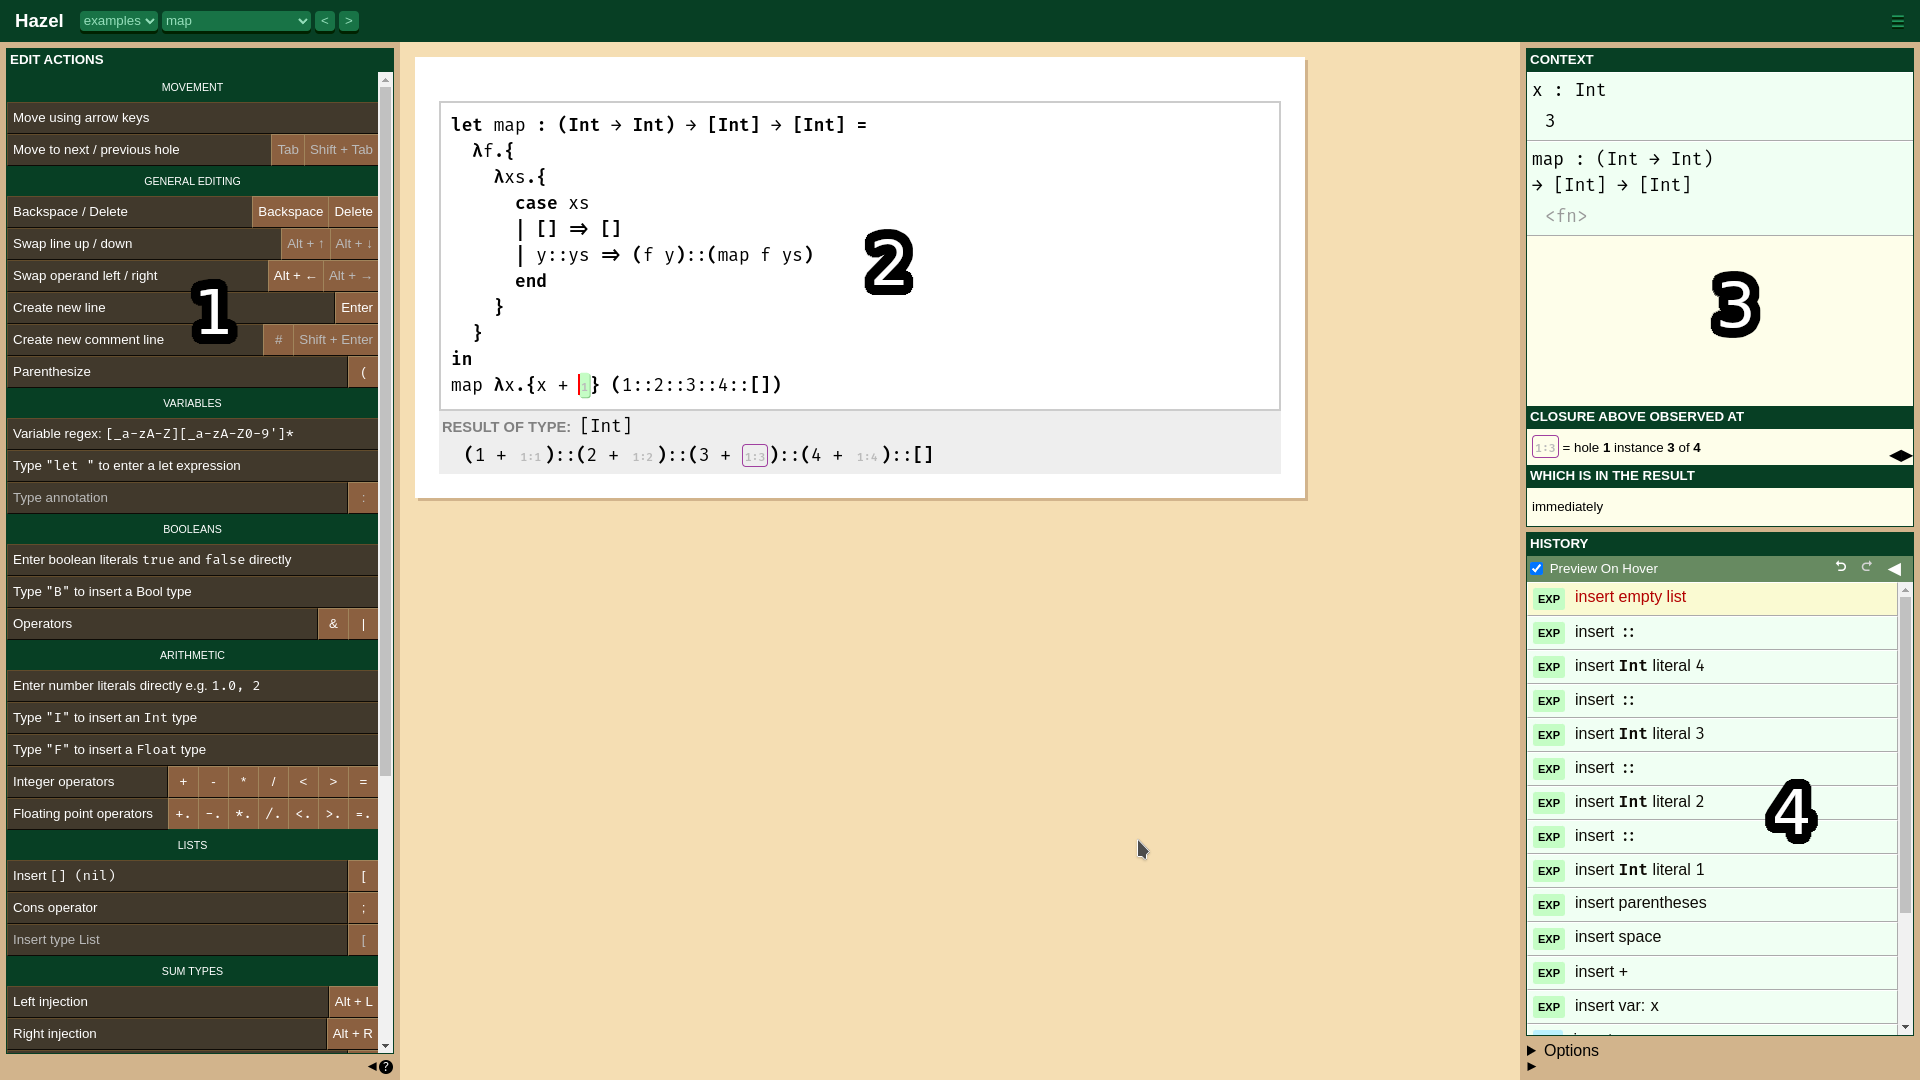
\includegraphics[width=\linewidth]{img/hazel_ui_annot.png}
  \caption{The Hazel interface, annotated}
  \label{fig:hazel-interface}
\end{figure}

\subsection{Implications of Hazel}
\label{sec:hazel-implications}

The main proposed use case of Hazel is its use in programming education, particularly for teaching functional programming, as it provides much useful feedback to the programmer for error conditions, allowing them to focus instead on semantic errors in their algorithm. This is being explored with the Hazel Tutor project \cite{potter2020hazel}.

Another research direction is in its use as a structural and graphical editor. For example, live GUIs \cite{omar2021filling} are being explored to enhance the editing experience by providing live, compositional, graphical interfaces, in addition to the benefits that Hazel's core calculi provide.

The result of a Hazel evaluation may contain holes, and thus not be fully evaluated. The Hazelnut Live paper \cite{conf/popl/HazelnutLive19} suggests the idea of hole-filling: since each hole in the result contains its lexical environment, we may ``resume'' evaluation without restarting evaluation from the beginning if a hole is filled -- this property is similar to that of computational notebooks. The problem with notebook execution is that it is stateful and running operations out-of-order may cause irreversible state changes that cause irreproducible results. On the other hand, resuming an evalution with fill-and-resume will produce the same result as if the program was run ordinarily from start to finish\footnote{This is a property known as \textit{commutativity} and described in \cite{conf/popl/HazelnutLive19}.} while avoiding re-evaluation of previous sections.

\section{Introduction to OCaml and Reason syntax}
\label{sec:ocaml-intro}

Previously, we have been introducing concepts using a pseudo-mathematical notation. When describing Hazel and its implementation, it may be useful to use sample code or pseudocode from the implementation to describe various aspects of Hazel.

Hazel is implemented in Reason (alternatively, ReasonML), which is a dialect of OCaml that offers a JavaScript-like syntax. Except for code samples in \Cref{app:code-samples}, the notation used throughout this report will be limited to referring to function names and types. Module names are denoted \texttt{PascalCase}, whereas function and type names are \texttt{snake\_case}. Conventionally, OCaml modules that export a type export a single type called \texttt{t}. As an example, \mintinline{ocaml}|DHExp.t| refers to the primarily-relevant type from the \mintinline{ocaml}|DHExp| module, the type that represents internal expressions $d$. On the other hand, \mintinline{ocaml}|Evaluator.evaluate| refers to the \mintinline{ocaml}|evaluate| function in the \mintinline{ocaml}|Evaluator| module. All functions and types will be prefixed with their module names for clarity.

\section{Hazel semantics}
\label{sec:hazel-semantics}

Hazel is rigorously defined using a bidirectional semantics. A high-level overview of the foundational papers on Hazelnut (syntax and static semantics) and Hazelnut Live (elaboration and dynamic semantics) is provided here, but a thorough explanation is deferred to the original papers.

\subsection{Hazelnut syntax}
\label{sec:hazel-syntax}

The grammar of Hazel's external language is defined as follows.

\begin{singlespace}
  \begin{align*}
    \tau &::= \tau\to\tau
           \mid b
           \mid \tehole \\
    e &::= c
        \mid x
        \mid\lambda x:\tau.e
        \mid e\ e
        \mid e:\tau
        \mid \hehole
        \mid \hhole{e}
  \end{align*}
\end{singlespace}

This is very similar to \gtlc{}. The $\gtlch{}$ type is rewritten as $\tehole$ and pronounced the ``hole type.'' An expression form for type ascription is added. Most notably, there is the addition of empty and non-empty expression holes, which are denoted $\hehole$ and $\hhole{e}$, respectively.

\subsection{Hazelnut action and typing semantics}
\label{sec:hazel-statics}

Hazelnut \cite{conf/popl/Hazelnut17} defines a bidirectional typing judgment for the external language. \todo{reproduce this in an appendix} The judgments are very similar to \gtlc{}. Unsurprisingly, hole expressions synthesize the hole type, and they analyze against any type. Note that in the case of a non-empty hole, the encapsulated expression must still synthesize a type, i.e., they are well-typed.

Hazelnut defines an action semantics for the structural editor, which describes the behavior of editing and maneuvering around a program. A program's edit state comprises an external expression with a superimposed cursor. There are four main actions carried out by the user: \texttt{move}, \texttt{construct}, and \texttt{delete}. These actions are described by bidirectionally-typed action judgments that transform a (well-typed) edit state to another (well-typed) edit state. There are a number of metatheorems that enforce desirable properties of action semantics in a structural editor, such as \textit{sensibility} (the result of an action on a well-typed expression is a well-typed expression), \textit{movement erase invariance} (movement actions should not change the external expression, but only the position of the cursor), \textit{reachability} (the cursor should be able to move to any valid location to any other valid location), \textit{constructability} (every valid edit state should be constructable from the initial edit state), \textit{action determinism} (every sequence of edit actions should have only one valid output state), etc. These metatheorems are proved using the Agda theorem proving assistant \cite{agda2017}.

\todo{talk about missing forms from the Hazelnut formulation: let expressions, case expressions, binary sum types, lists, other hole types, fixpoint}

\subsection{Hazelnut Live elaboration judgment}
\label{sec:hazel-elaboration}

\textit{Elaboration} is the process of converting an expression from the external language to the internal language. Notably, both the external and internal languages share the same type system. The internal language and the elaboration process is very similar to the cast calculus \gtclc and the elaboration process from \gtlc.

The elaboration algorithm is also bidirectionally-typed, and thus involves two mutually-recursive judgments: a \textit{synthetic elaboration judgment} $\Gamma^-\vdash e^-\Rightarrow\tau^+\leadsto d^+\dashv\Delta^+$, and an \textit{analytic elaboration judgment} $\Gamma^-\vdash e^-\Leftarrow\tau^-\leadsto d^+:\tau'^+\dashv\Delta^+$.\todo{reproduce elaboration judgments in appendix}

$\Delta$ is the \textit{hole context}, used to store the typing context and actual type of each hole. Each hole (whether in synthetic or analytic position) is recorded in the hole context, and is given the identity mapping as its original environment\footnote{This is amended in this work, in which holes will not initially be given an environment because the environment is not substitution-based.}.

The elaboration judgment will produce as output a type for the internal expression, which may be different from the type of the external expression. In particular, elaborated holes will produce different types depending on whether they are in synthetic or analytic position.

\subsection{Hazelnut Live final judgment and dynamic semantics}
\label{sec:hazel-dynamics}

Hazelnut Live introduces a new $d\textsf{ final}$ judgment for the internal language, used to indicate an irreducible expression. This subsumes the set of fully-evaluated expressions in \gtclc, which include plain values or \textit{boxed values}, values which are casted ``out'' of their original type but not yet casted ``into'' the destination type. However, expressions containing holes also cannot further evaluate and comprise the second class of final expressions: \textit{indeterminate} values.

\todo{reproduce final judgment}

Hazelnut Live defines a small-step semantics for its internal language very similar to that of \gtclc. To avoid the rapid proliferation of rules due to the small-step semantics, a notational convenience called the \textit{evaluation context} $\mathcal{E}$, which recursively evaluates subexpressions. The rules are modified to accomodate indeterminate expressions.

\todo{reproduce small-step semantics in an appendix}

\subsection{Hole instance numbering}
\label{sec:hole-instance-numbering}

Hazelnut Live introduces \textit{hole instances} with some motivation, but with no details of its implementation. In \Cref{sec:renumbering}, we will motivate hole instances in greater detail, describe the current implementation, and reformulate the problem of hole instance tracking to accomodate environments and memoization.

%%% Local Variables:
%%% mode: latex
%%% TeX-master: "main"
%%% End:

\section{Implementing the environment model of evaluation}
\label{sec:env_model_evaluation}

\subsection{Hazel-specific implementation}
\label{sec:eval_with_envs}

In the case of Hazel (which does not prioritize speed of evaluation in its implementation, and is not a compiled language), evaluation with (reified) environments offers an additional (performance) benefit over the substitution model: the ability to easily identify (and thus memoize) operations over environments. This is useful for the optimizations described later in this paper.

The implementation of evaluation in Hazel differs from a typical interpreter implementation of evaluation with environments in three regards: we need to account for hole environments; environments are uniquely identified by an identifier for memoization (in turn for optimization); and any closures in the evaluation result should be converted back into plain $\lambda$ abstractions.

\subsubsection{Evaluation rules}
\label{sec:evalenv-rules}

% TODO: walk through simple example

Omar et al. \cite{conf/popl/HazelnutLive19} describes evaluation with the substitution model using a little-step semantics with an evaluation context $\mathcal{E}$. 

The Hazel implementation follows a big-step model for evaluation, which is simpler, more performant, and does not require the evaluation context. Thus it is more convenient to follow a big-step semantics as shown in \Cref{fig:big-step-formal}. An equivalent small-step semantics is described in \Cref{sec:small-step-evalenv} but will not be discussed further.

The evaluation model threads a run-time environment $\env$\footnote{The symbol $\env$ was chosen to represent the environment as it was used to represent hole environments in \cite{conf/popl/HazelnutLive19}. The relationship between these two environments will be discussed in \Cref{sec:holeenv_evalenv_connection}.} throughout the evaluation process. An environment is conceptually a mapping $\env:x\mapsto d$, although it will later be augmented to be more amenable to memoization.

% TODO: closure conversion
% TODO: move discussion of closure conversion to background section

% TODO: introduce big-step formalization
\begin{figure}
  \centering
  \begin{mdframed}
    \begin{singlespace}
      \judgbox{E\vdash d\Downarrow d'}{Internal expression $d$ evaluates to $d'$ given environment $E$}

\begin{mathpar}
  \Infer{EvalB-Final}{E\vdash d\textsf{ final}}{E\vdash d\Downarrow d}
  \and
  \Infer{EvalB-Var}{}{E,x\leftarrow d\vdash x\Downarrow d}
  \and
  \Infer{EvalB-Lam}{
    [\hhole{d''}_{\sigma}/\hhole{d''}_{\sigma::E}][\hehole_{\sigma}/\hehole_{\sigma::E}]d=d'
  }{E\vdash(\lambda x:\tau.d)\Downarrow [E](\lambda x:\tau.d')}
  \and
  \Infer{EvalB-Ap$_1$}{
    E\vdash d_1\Downarrow d_1' \\
    d_1'\ne([E']\lambda x:\tau.d) \\
    E\vdash d_2\Downarrow d_2'
  }{E\vdash d_1(d_2)\Downarrow d_1'(d_2')}
  \and
  \Infer{EvalB-Ap$_2$}{
    E\vdash d_1\Downarrow ([E']\lambda x:\tau.d_1') \\
    E\vdash d_2\Downarrow d_2' \\
    E::E',x\leftarrow d_2'\vdash d_1'\Downarrow d
  }{E\vdash d_1(d_2)\Downarrow d}
  \and
  \Infer{EvalB-Let}{
    E\vdash d_2\Downarrow d_2' \\
    E,x\leftarrow d_2'\vdash d_1\Downarrow d
  }{E\vdash\texttt{let }x=d_2\texttt{ in }d_1\Downarrow d}
  \and
  \Infer{EvalB-Op$_1$}{
    E\vdash d_1\Downarrow d_1' \\
    E\vdash d_2\Downarrow d_2' \\
    (d_1\ne\hnum{n_1}\lor d_2\ne\hnum{n_2})
  }{E\vdash d_1+d_2\Downarrow d_1'+d_2'}  
  \and
  \Infer{EvalB-EHole}{}{E\vdash\hehole_{\sigma}\Downarrow\hehole_{\sigma::E}}
  \and
  \Infer{EvalB-NEHole}{
    E\vdash d\Downarrow d'
  }{E\vdash\hhole{d}_{\sigma}\Downarrow\hhole{d'}_{\sigma::E}}
  \and
  \Infer{EvalB-Op$_2$}{
    E\vdash d_1\Downarrow\hnum{n_1} \\
    E\vdash d_2\Downarrow\hnum{n_2}
  }{E\vdash d_1+d_2\Downarrow\hnum{n_1+n_2}}
\end{mathpar}

%%% Local Variables:
%%% mode: latex
%%% TeX-master: "main"
%%% End:

    \end{singlespace}
  \end{mdframed}
  \caption{Big-step semantics for the environment model of evaluation}
  \label{fig:big-step-formal}
\end{figure}

% TODO: describe formalization
% TODO: describe the implementation

\subsubsection{Connection to hole environments}
\label{sec:holeenv_evalenv_connection}

\subsubsection{Differences to the substitution model of evaluation}
\label{sec:differences_subst}

\subsection{The evaluation boundary and post-processing}
\label{sec:closures_to_lambdas}


% TODO: describe why the result from substitution is better than the result from environments

% TODO: example programs:
% - lambda and fix forms
% - holes inside and outside boundary
% - recursion through hole environments

% two-stage approach

\begin{figure}
  \centering
  \begin{mdframed}
    \begin{singlespace}
      \judgbox{\env\vdash d\pplc d'}{$d$ postprocesses ($\lambda$-conversion) to $d'$ outside the evaluation boundary}

\begin{mathpar}
  \Infer{\pplclo-Value}{
    d\textsf{ value} \\
    d\ne\lambda x.d
  }{d\pplc d}
  \and
  \Infer{\pplclo-Var}{}{\env,x\leftarrow d\vdash x\pplc d}
  \and
  \Infer{\pplclo-Fix}{
    \env\vdash d\pplc d'
  }{\env\vdash\fix f.d\pplc\fix f.d'}
  \and
  \Infer{\pplclo-Lam}{
    \env\vdash d\pplc d'
  }{\env\vdash\lambda x.d\pplc\lambda x.d'}
  \and
  \Infer{\pplclo-Ap}{
    \env\vdash d_1\pplc d_1' \\
    \env\vdash d_2\pplc d_2'
  }{\env\vdash d_1(d_2)\pplc d_1'(d_2')}
  \and
  \Infer{\pplclo-Op}{
    \env\vdash d_1\pplc d_1' \\
    \env\vdash d_2\pplc d_2'
  }{\env\vdash d_1+d_2\pplc d_1'+d_2'}
  \and
  \Infer{\pplclo-EHole}{
  }{\env\vdash\hehole_\varnothing^u\pplc\hehole_\env^u}
  \and
  \Infer{\pplclo-NEHole}{
    \env\vdash d\pplc d'
  }{\env\vdash\hhole{d}_\varnothing^u\pplc\hhole{d'}_\env^u}
\end{mathpar}

\judgbox{d\pplc d'}{$d$ postprocesses ($\lambda$-conversion) to $d'$ within the evaluation boundary}

\begin{mathpar}
  \Infer{\pplcl-Value}{
    d\textsf{ value} \\
    d\ne\fix f.d \\
    d\ne [\env]\lambda x.d
  }{d\pplc d}\\
  \and
  \Infer{\pplcl-Fix}{
    \env\vdash d\pplc d'\\
    \env,f\leftarrow (\fix f.\lambda x.d')\vdash d'\pplc d''
  }{\fix f.([\env]\lambda x.d)\pplc \lambda x.d''}
  \and
  \Infer{\pplcl-Closure}{
    \env\vdash d\pplc d'
  }{[\env]\lambda x.d\pplc\lambda x.d'}
  \and
  \Infer{\pplcl-Ap}{
    d_1\pplc d_1' \\
    d_2\pplc d_2'
  }{d_1(d_2)\pplc d_1'(d_2')}
  \and
  \Infer{\pplcl-Op}{
    d_1\pplc d_1' \\
    d_2\pplc d_2'
  }{d_1+d_2\pplc d_1'+d_2'}
  \and
  \Infer{\pplcl-EHole}{
    \env'=\{(x\leftarrow d'):(x\leftarrow d)\in\env,d\pplc d'\}
  }{\hehole_\env^u\pplc\hehole_{\env'}^u}
  \and
  \Infer{\pplcl-NEHole}{
    d\pplc d' \\
    \env'=\{(x\leftarrow d'):(x\leftarrow d)\in\env,d\pplc d'\}
  }{\hhole{d}_\env^u\pplc\hhole{d'}_{\env'}^u}
\end{mathpar}

TODO: closure needs to go recursive

%%% Local Variables:
%%% mode: latex
%%% TeX-master: "main"
%%% End:

    \end{singlespace}
  \end{mdframed}
  \caption{Big-step semantics for $\lambda$-conversion post-processing}
  \label{fig:big-step-inside-formal}
\end{figure}

\subsection{A strict evaluation boundary}
\label{sec:strict_eval_boundary}

% TODO: example program: pattern doesn't match

\subsection{Post-processing memoization}
\label{sec:memoization}

\subsubsection{Modifications to the environment datatype}
\label{sec:memoization-evalenv}

\subsubsection{Modifications to the post-processing rules}
\label{sec:memoization-postprocessing}

\begin{figure}
  \centering
  \begin{mdframed}
    \begin{singlespace}
      \judgbox{TODO}{TODO}

\begin{mathpar}
  TODO
\end{mathpar}

%%% Local Variables:
%%% mode: latex
%%% TeX-master: "main"
%%% End:

    \end{singlespace}
  \end{mdframed}
  \caption{Big-step semantics modifications for environment memoization}
  \label{fig:big-step-memoization-rules}
\end{figure}

\subsection{Purity}
\label{sec:env-purity}

% threading around state: technically still pure, represented very similar to rules
% evalenv number generation is threaded around very similar to metavargen, but
% somewhat unwieldy and 

\subsubsection{Elegance and complexity of implementation}
\label{sec:elegance-and-complexity}

% purity is a technical term, elegance is not; unwieldiness
% is the additional complexity worth it?
% - nice benefits with memoization in specific cases (will see later)
% - general linear speedup even with the overhead and without benefits of memoization
% (e.g., see Fibonacci example)

%%% Local Variables:
%%% mode: latex
%%% TeX-master: "main"
%%% End:

\section{Implementation and optimization of FAR}
\label{sec:far_impl}

\subsection{Evaluation with environments}
\label{sec:eval_with_envs}

\subsection{Restructuring hole numbering}
\label{sec:restructuring_hole_numbering}

\subsection{Implementing FAR}
\label{sec:implementing_far}

\subsection{Memoization of recent actions}
\label{sec:memoization_actions}

\subsection{UI changes for notebook-like editing}
\label{sec:notebook_ui}

%%% Local Variables:
%%% mode: latex
%%% TeX-master: "main"
%%% End:

\chapter{Evaluation of performance}
\label{sec:evaluation}

To evaluate performance, benchmarks were carried out using the \mintinline{ocaml}|TimeUtil.measure_time| utility. Benchmarks were carried out on Google Chrome 99 on Debian 10 on an Intel i3-2100 CPU. The times shown are a mean of three trials. Evaluation step counts are tracked in \mintinline{ocaml}|EvalState.t| and count the number of calls to \mintinline{ocaml}|Evaluator.evaluate| as described in \Cref{sec:step-counting}.

There are a number of factors that may affect the consistency of the elapsed time benchmarks. Such factors include the quality of JSOO-generated Javascript, specifics of the Chrome V8 Javascript engine, inaccuracies in the Javascript timing function, and random system fluctuations.

\section{Evaluation performance using the environment model}
\label{sec:evaluation-evalenv}

To evaluate the performance of evaluation using the environment model, we benchmark the performance of a computationally-expensive function, the tree-recursive Fibonacci function. This function is chosen because it is computationally expensive and does not have a deep recursion depth\footnote{This is because Hazel does not implement TCO, and thus would overflow the stack with too much (tail-)recursion.}. It is also a complete program, i.e., it does not have holes and the hole renumbering and postprocessing steps are not of concern here.

We try out a few variations of the $\text{fib}(n)$ function, shown in \Cref{fig:perf-fib}, for $n=\{22,23,24,25,26\}$. These numbers were chosen somewhat arbitrarily. They are large enough to allow for reproducible results, and small enough to prevent excessively long runtimes. The first variation is shown in \Cref{fig:perf-fib-more-bindings}, which involves more global variables. The second variation is shown in \Cref{fig:perf-fib-more-branches}, in which an additional branch is added. This branch is never taken (as the third rule's pattern will always match), and it involves some instances of the variable $f$.

For this experiment, the builtin variables and functions are removed. Restoring the builtins would be very similar to the second program variation.

The quantitative results of this experiment are shown in \Cref{tab:perf-fib-all}.

\begin{listing}
  \inputhminted{perf_fib}
  \caption{An evaluation-heavy Hazel program with no holes}
  \label{fig:perf-fib}
\end{listing}

\begin{listing}
  \inputhminted{perf_fib_more_bindings}
  \caption{Adding global bindings to the program in \Cref{fig:perf-fib}}
  \label{fig:perf-fib-more-bindings}
\end{listing}

\begin{listing}
  \inputhminted{perf_fib_more_branches}
  \caption{Adding variable substitutions to unused branches to the program in \Cref{fig:perf-fib}}
  \label{fig:perf-fib-more-branches}
\end{listing}

\begin{singlespace}
  \begin{table}
    \centering
    \begin{subtable}{\textwidth}
      \begin{tabular}{r|c|ccccc|ccccc}
        \hline
        & & \multicolumn{5}{c|}{Variables in unused branch} & \multicolumn{5}{c}{Extra global variables} \\
        n & Regular & 2 & 4 & 6 & 8 & 10 & 2 & 4 & 6 & 8 & 10 \\
        \hline\hline
        22 & 334 & 394 & 509 & 539 & 658 & 677 & 339 & 305 & 302 & 339 & 336 \\
        23 & 478 & 599 & 695 & 835 & 1116 & 1107 & 524 & 442 & 452 & 452 & 455 \\
        24 & 775 & 929 & 1214 & 1332 & 1518 & 1686 & 744 & 700 & 729 & 794 & 708 \\
        25 & 1233 & 1502 & 1874 & 2310 & 2398 & 2723 & 1171 & 1189 & 1134 & 1104 & 1231 \\
        26 & 2019 & 2391 & 2939 & 3399 & 3872 & 4417 & 1841 & 1747 & 1761 & 1773 & 1780 \\
        \hline\hline
      \end{tabular}
      \caption{\texttt{dev} branch}
      \label{tab:perf-fib-dev}
    \end{subtable} \\
    \vspace{1em}
    \begin{subtable}{\textwidth}
      \begin{tabular}{r|c|ccccc|ccccc}
        \hline
        & & \multicolumn{5}{c|}{Variables in unused branch} & \multicolumn{5}{c}{Extra global variables} \\
        n & Regular & 2 & 4 & 6 & 8 & 10 & 2 & 4 & 6 & 8 & 10 \\
        \hline\hline
        22 & 255 & 267 & 276 & 242 & 245 & 243 & 330 & 384 & 417 & 435 & 519 \\
        23 & 406 & 374 & 376 & 358 & 366 & 330 & 497 & 576 & 573 & 593 & 660 \\
        24 & 578 & 558 & 559 & 591 & 561 & 569 & 775 & 857 & 911 & 912 & 1037 \\
        25 & 851 & 883 & 871 & 864 & 888 & 908 & 1209 & 1363 & 1469 & 1473 & 1684 \\
        26 & 1318 & 1388 & 1382 & 1398 & 1399 & 1415 & 1935 & 2262 & 2302 & 2356 & 2492 \\
        \hline\hline
      \end{tabular}
      \caption{\texttt{eval-environment} branch}
      \label{tab:perf-fib-evalenv}
    \end{subtable}

    \caption{Time (ms) to compute $\text{fib}(n)$}
    \label{tab:perf-fib-all}
  \end{table}
\end{singlespace}

\begin{figure}
  \centering
  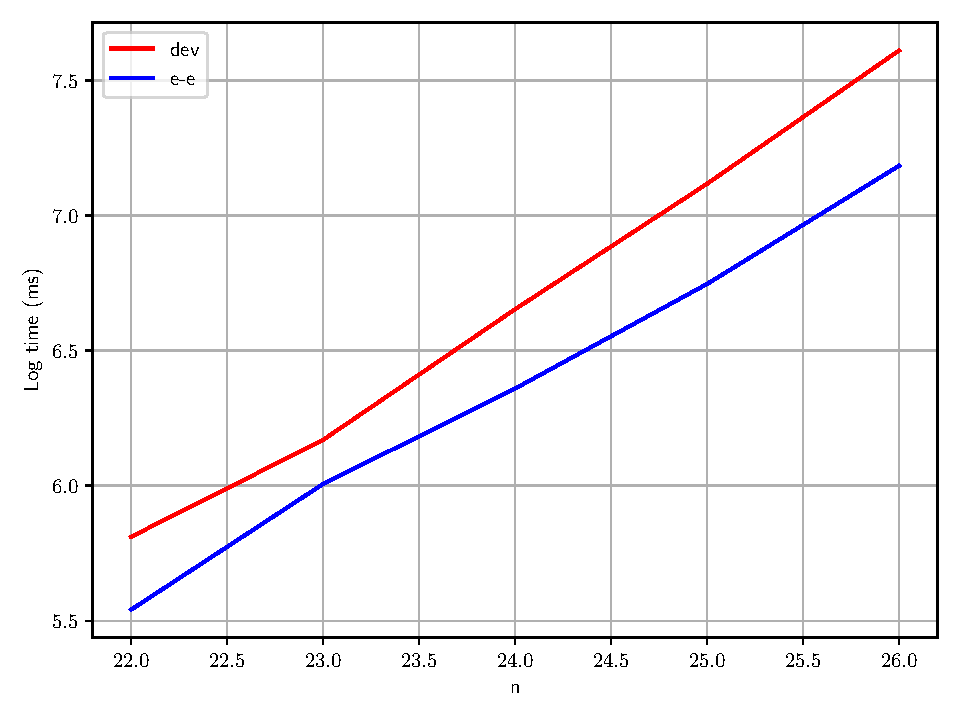
\includegraphics[width=0.7\textwidth]{img/perf_fib.pdf}
  \caption{Performance of evaluating $\text{fib}(n)$}
  \label{fig:perf-fib}
\end{figure}

\begin{figure}
  \centering
  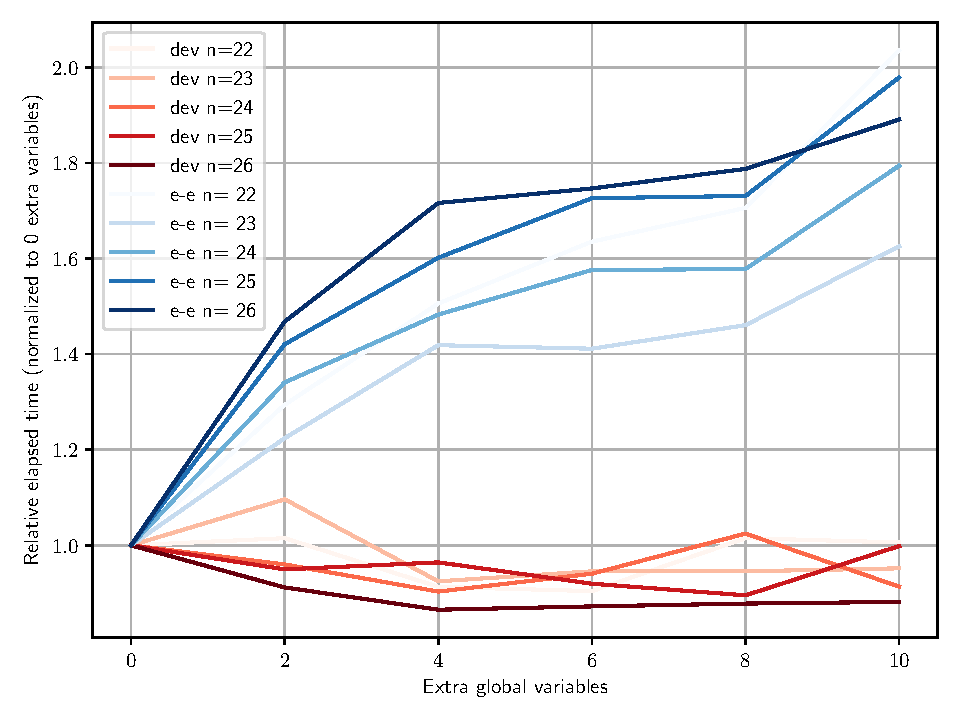
\includegraphics[width=0.7\textwidth]{img/perf_fib_more_vars.pdf}
  \caption{Performance of evaluating $\text{fib}(n)$ with extra global variables}
  \label{fig:perf-fib-more-vars}
\end{figure}

\begin{figure}
  \centering
  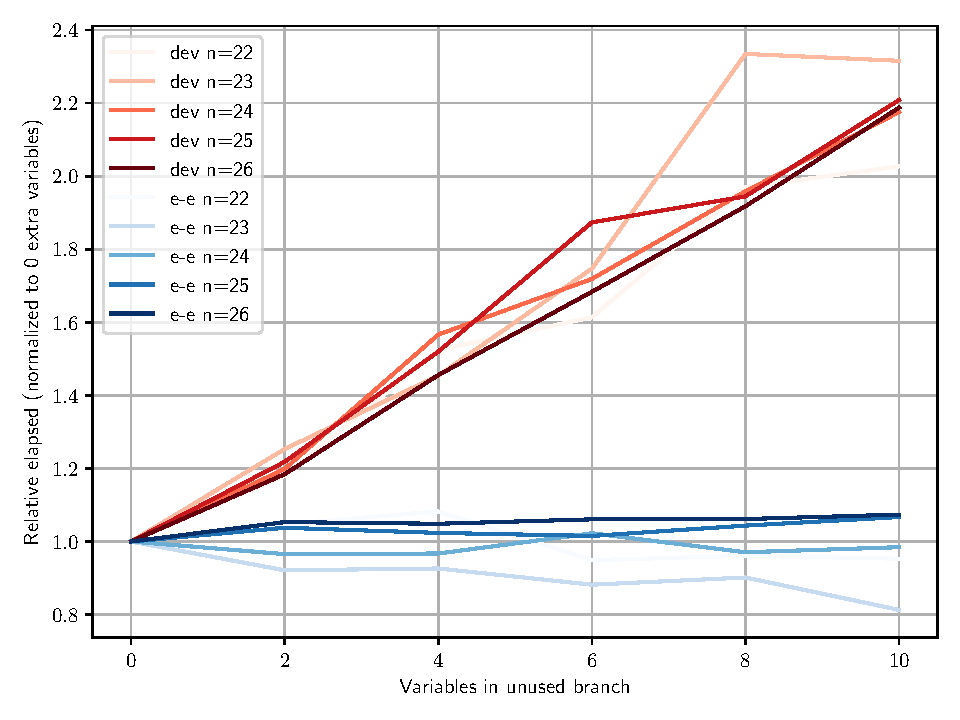
\includegraphics[width=0.7\textwidth]{img/perf_fib_more_branches.pdf}
  \caption{Performance of evaluating $\text{fib}(n)$ with an unused branch}
  \label{fig:perf-fib-more-branches}
\end{figure}


\section{Postprocessing performance}
\label{sec:evaluation-renumbering}

Consider the set of programs described by \Cref{fig:hole_renumbering_problem}.

\todo{describe this code blowup example}

\begin{singlespace}
  \begin{table}
    \centering
    \begin{tabular}{r|ccc|ccc}
      \hline
      & \multicolumn{3}{c|}{\texttt{dev} branch} & \multicolumn{3}{c}{\texttt{eval-environment} branch} \\
      & Evaluate & Postprocessing & Equality & Evaluate & Postprocessing & Equality \\
      \hline\hline
      1 & 0 & 0 & 0 & 0 & 1 & 0 \\
      2 & 0 & 0 & 0 & 0 & 1 & 0 \\
      3 & 1 & 2 & 0 & 0 & 1 & 0 \\
      4 & 1 & 1 & 1 & 1 & 0 & 0 \\
      5 & 1 & 1 & 2 & 0 & 3 & 0 \\
      6 & 5 & 1 & 3 & 1 & 0 & 0 \\
      7 & 4 & 5 & 6 & 2 & 2 & 0 \\
      8 & 3 & 3 & 14 & 0 & 0 & 0 \\
      9 & 6 & 18 & 33 & 1 & 0 & 1 \\
      10 & 14 & 29 & 61 & 0 & 0 & 0 \\
      11 & 13 & 41 & 91 & 3 & 2 & 0 \\
      12 & 25 & 145 & 203 & 2 & 0 & 1 \\
      13 & 65 & 578 & 383 & 2 & 0 & 0 \\
      14 & 147 & 2399 & 924 & 1 & 3 & 1 \\
      15 & 226 & 16597 & 1603 & 3 & 0 & 1 \\
      16 & & & & 1 & 0 & 1 \\
      17 & & & & 2 & 1 & 1 \\
      18 & & & & 0 & 3 & 1 \\
      19 & & & & 0 & 0 & 1 \\
      20 & & & & 3 & 4 & 0 \\
      21 & & & & 2 & 0 & 1 \\
      22 & & & & 0 & 2 & 1 \\
      23 & & & & 0 & 3 & 1 \\
      24 & & & & 0 & 6 & 1 \\
      25 & & & & 1 & 4 & 1 \\
      26 & & & & 1 & 2 & 1 \\
      \hline\hline
    \end{tabular}
    \caption{Performance of program illustrated in \Cref{fig:hole_renumbering_problem}}
    \label{tab:perf-hole-blowup}
  \end{table}
\end{singlespace}

\begin{figure}
  \centering
  \begin{subfigure}{0.7\textwidth}
    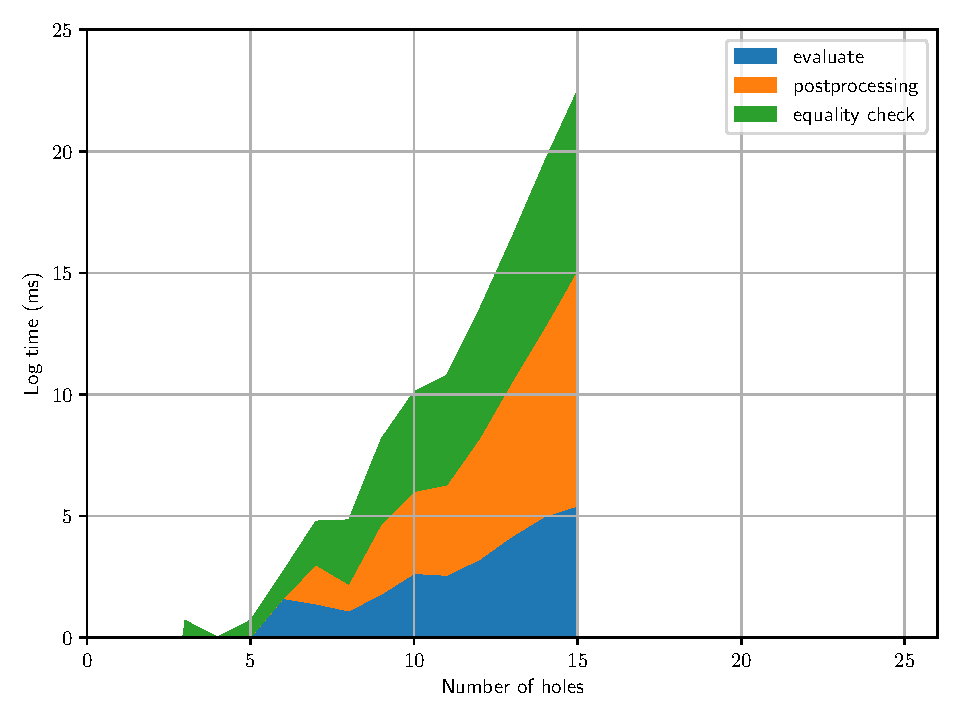
\includegraphics[width=\textwidth]{img/perf_renum_dev.pdf}
    \caption{\texttt{dev} branch}
    \label{fig:perf-renum-dev}
  \end{subfigure}
  \begin{subfigure}{0.7\textwidth}
    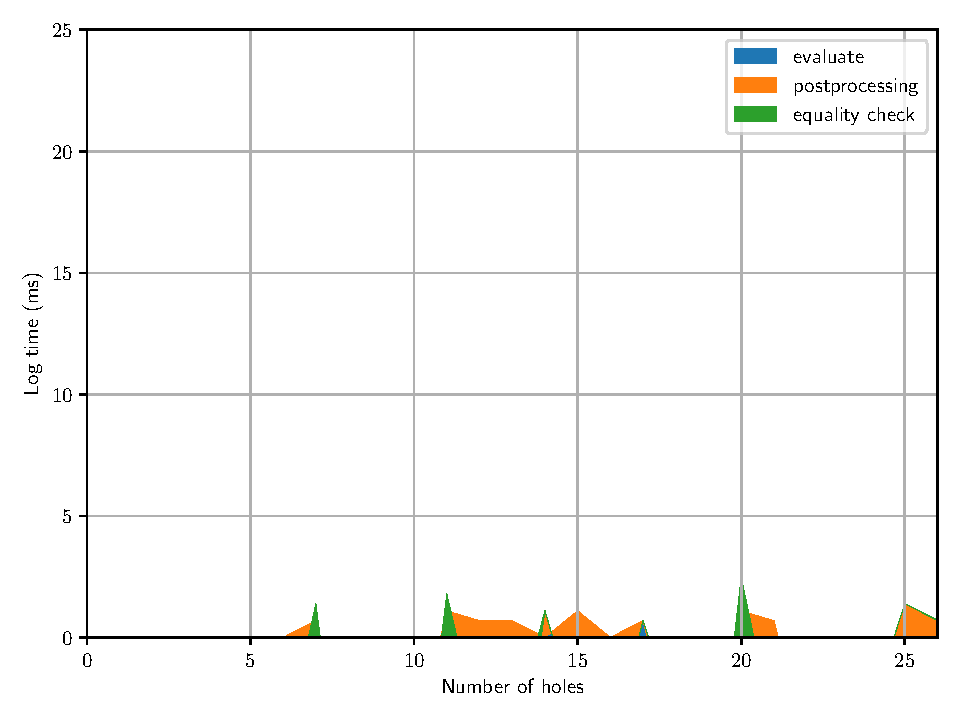
\includegraphics[width=\textwidth]{img/perf_renum_eev.pdf}
    \caption{\texttt{eval-environment} branch}
    \label{fig:perf-renum-eev}
  \end{subfigure}
  \caption{Performance of evaluating program in \Cref{fig:hole_renumbering_problem}}
  \label{fig:perf-renum}
\end{figure}

\section{FAR performance}
\label{sec:evaluation-far}

\begin{singlespace}
  \begin{table}
    \centering
    \begin{tabular}{p{10em}cccc}
      \hline
      Program & Steps & Steps & Step $\Delta$ & Cumulative \\
              & & (w/ FAR) & & Step $\Delta$ \\
      \hline\hline
      \inputhnfminted{far_fib_hist_1} & 7 & - & 0 & 0 \\ \hline
      \inputhnfminted{far_fib_hist_2} & 12 & 21 & 9 & 9 \\ \hline
      \inputhnfminted{far_fib_hist_3} & 17 & - & 0 & 9 \\ \hline
      \inputhnfminted{far_fib_hist_4} & 58 & 69 & 11 & 20 \\ \hline
      \inputhnfminted{far_fib_hist_5} & 4762964 & - & 0 & 20 \\ \hline
      \inputhnfminted{far_fib_hist_6} & 4762966 & 12 & -4762954 & -4762934 \\ \hline
      \inputhnfminted{far_fib_hist_7} & 4762966 & 21 & -4762954 & -9525879 \\ \hline
      \inputhnfminted{far_fib_hist_8} & 4792967 & 13 & -4792954 & -14288813 \\ \hline
      \hline
    \end{tabular}
    \caption{A program edit history with an expensive computation}
    \label{fig:far-program-history-fib}
  \end{table}
\end{singlespace}

\begin{singlespace}
  \begin{table}
    \centering
    \begin{tabular}{p{10em}cccc}
      \hline
      Program & Steps & Steps & Step $\Delta$ & Cumulative \\
              & & (w/ FAR) & & Step $\Delta$ \\
      \hline\hline
      \inputhnfminted{far_hist_1} & 1 & - & 0 & 0 \\ \hline
      \inputhnfminted{far_hist_2} & 2 & 3 & 1 & 1 \\ \hline
      \inputhnfminted{far_hist_3} & 3 & - & 0 & 1 \\ \hline
      \inputhnfminted{far_hist_4} & 4 & 5 & 1 & 2 \\ \hline
      \inputhnfminted{far_hist_5} & 5 & - & 0 & 2 \\ \hline
      \inputhnfminted{far_hist_6} & 6 & 9 & 3 & 5 \\ \hline
      \inputhnfminted{far_hist_7} & 8 & 8 & 0 & 5 \\ \hline
      \inputhnfminted{far_hist_8} & 9 & 14 & 5 & 10 \\ \hline
      \inputhnfminted{far_hist_9} & 10 & 11 & 1 & 11 \\ \hline
      \inputhnfminted{far_hist_10} & 11 & 6 & -5 & 6 \\ \hline
      \hline
    \end{tabular}
    \caption{A sample edit history for a simple program}
    \label{fig:far-program-history-simple}
  \end{table}
\end{singlespace}

\begin{figure}
  \centering
  \begin{subfigure}{0.7\textwidth}
    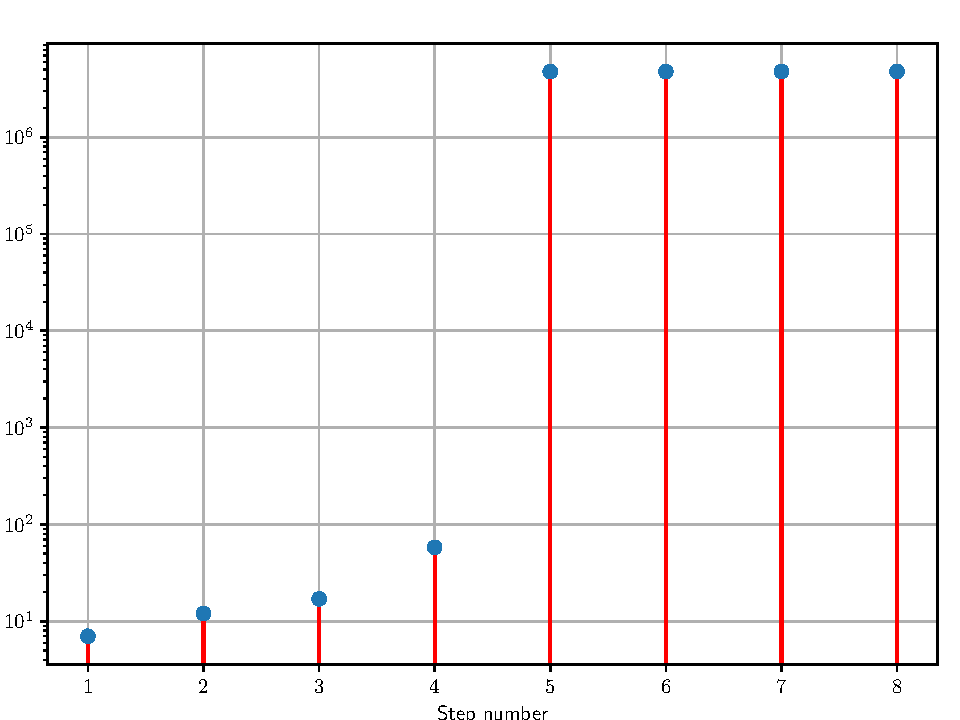
\includegraphics[width=\textwidth]{img/perf_no_far.pdf}
    \caption{Normal evaluation}
    \label{fig:perf-no-far}
  \end{subfigure}
  \begin{subfigure}{0.7\textwidth}
    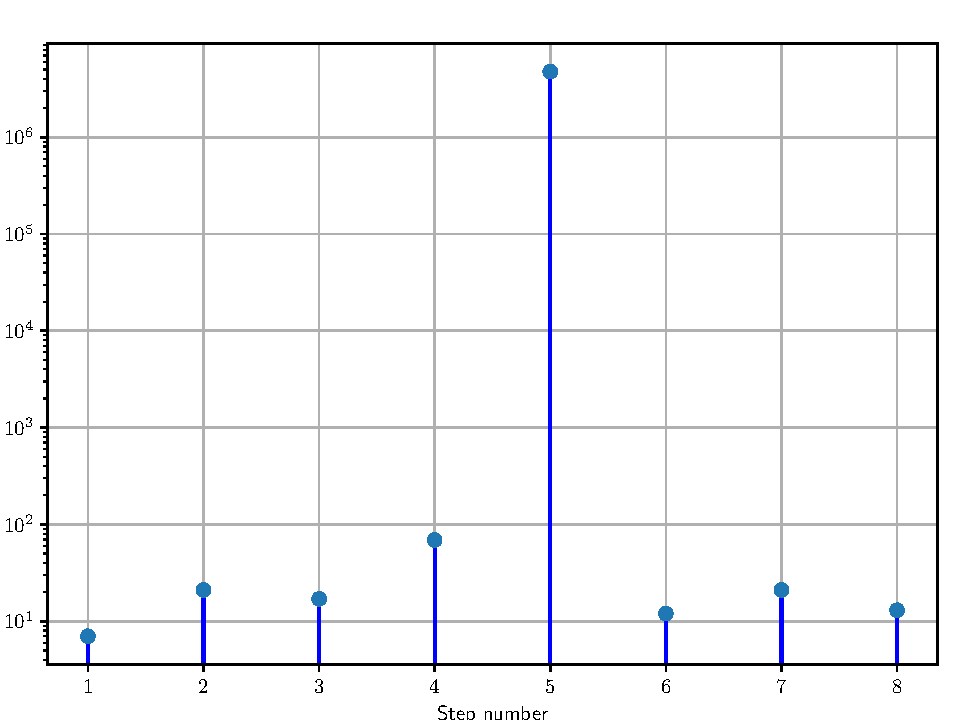
\includegraphics[width=\textwidth]{img/perf_far.pdf}
    \caption{With one-step FAR}
    \label{fig:perf-far-far}
  \end{subfigure}
  \caption{Number of evaluation steps per edit in \Cref{fig:far-program-history-fib}}
  \label{fig:perf-far}
\end{figure}

%%% Local Variables:
%%% mode: latex
%%% TeX-master: "main"
%%% End:

\chapter{Future work}
\label{sec:future_work}

\section{Simplification of the postprocessing algorithms}
\label{sec:postprocessing-simplification}

The postprocessing algorithms presented in \Cref{sec:postprocessing-substitution,sec:hole-numbering-algorithm} are both memoized to avoid repeatedly postprocessing an environment multiple times. However, the latter algorithm (hole numbering) complicates memoization. This is due to the fact that holes need to be re-postprocessed each time it is encountered in a new parent in order to track the closure parents.

It would be desirable if we can avoid working around this, perhaps by reformulating the way hole parents are tracked. A possible solution is to implementing hole parent tracking as a separate postprocessing pass after hole closure numbering.

\section{Improvements to FAR}
\label{sec:far-improvements}

\subsection{Finishing the implementation of FAR}
\label{sec:finishing-far}

The implementation of FAR completed for this thesis is a limited proof-of-concept. The FAR detection mechanism (the structural diffing algorithm) and preprocessing steps are complete. However, due to limited time constraints, the implementation has not achieved parity with the theoretical exploration of FAR explored in this paper.

\begin{itemize}
\item A list of past edit states should be made accessible to the FAR detection algorithm. The current structure of the Hazel toplevel and the undo history makes this a little trickier because there may be multiple unrelated histories caused by switching programs (``cards'') in the top panel of the Hazel UI.
\item The result of FAR should be memoized alongside the results from regular evaluation. The current implementation of normal evaluation is memoized and is not aware of the FAR operation.
\item The result of evaluating the program (\mintinline{ocaml}|Result.t|) is not currently stored in the model, but the program's edit state (\mintinline{ocaml}|Program.t|) is. This means that when the program result is needed in the Hazel UI, the program is re-evaluated. This is usually not a problem because of memoization, but FAR results are not memoized. It would be better to store the results of evaluation in the model and undo history to avoid this trouble.
\item There is a slight issue with the current description of the \mintinline{ocaml}|FillExp| variant $\hhole{d}_i$. This requires us to have access to the hole closure identifier $i$, which comes from the postprocessed result. However, we perform the FAR operation on the un-postprocessed result. To remedy this, we may begin evaluation from the post-processed result, which may cause us to change some of our assumptions about the evaluation boundary. Another solution would be to have an alternative postprocessing operation that renumbers holes but leaves alone the evaluation boundary.
\end{itemize}

\subsection{Memoization for environments during re-evaluation}
\label{sec:far-improv-memo-envs}

We introduced fill expressions $\hhole{d}_i$ in \Cref{sec:far-preprocessing} in order to memoize the evaluation of filled expressions during re-evaluation.

It will also be beneficial to memoize the re-evaluation of closure environments. To illustrate why this is the case, consider the case of \Cref{fig:far-hole-closure-memoization}. In this example, the environment is evaluated twice, even though it is the same physical environment. Each environment will be re-evaluated each time it is encountered, leading to the same exponential blowup problem encountered when dealing with postprocessing in \Cref{fig:hole_renumbering_problem}. The implementation of this memoization is the same as before; we will need a new environment state variable mapping environment identifiers to evaluated environments.

\subsection{Choosing the edit state to fill from}
\label{sec:far-past-edit-states}

There are a number of possible design decisions when searching for a valid hole fill. Firstly, one must decide the maximum number of edit states to search: should it be a fixed number of edit states, or should it be given a fixed time budget? Is it best to cache edit states that recently led to a fill operation (\`a la LRU cache)? Is the most recent edit state that leads to a valid fill usually the best candidate, or even a good candidate? Would it be best to allow for user-configurable settings, or perhaps even for the user to manually select the previous edit from which to fill?

It will be useful to collect empirical data about user-editing behaviors, as discussed in \Cref{sec:collect-edit-statistics}, in order to better tune these parameters. Alternatively, we may allow for some user configuration of FAR, as discussed in \Cref{sec:far-improv-user-config}.

\subsection{User-configurable FAR}
\label{sec:far-improv-user-config}

The FAR procedure as described is a completely automatic process. However, the choice of which past edit state to choose may be tricky, as described in \Cref{sec:far-past-edit-states}. It may be desirable for the user to manually set a past edit state as an ``anchor'' from which to set FAR, and thus override an automatic choice of past edit state. This reifies the concept of sections or section breaks from computational notebooks. However, since a user-chosen edit state may not lead to a valid fill diff, edit states that lead to an invalid fill diff will still have to be evaluated from scratch.

It may also be desirable to disable FAR completely, whether for debugging purposes or because it does not help performance much in the given circumstance. This should be a toggleable parameter in the sidebar.

\subsection{UI changes for notebook-style evaluation}
\label{sec:far-improv-notebook-ui}

We have motivated the use of Hazel with FAR for notebook-style evaluation in \Cref{sec:notebook-ui}. It may be useful to the programmer to have additional visual aids to help enforce the benefits of resumed evaluation.

It may be useful to format the code editor using a series of sections. These sections will be syntactic sugar for sequences of let statements, and edits to the code in a section will only cause the current and subsequent sections to re-evaluate. This also presents a method to choose the edit state from which to fill that is intuitive to the user.

Another useful feature to evaluate FAR is to show evaluation statistics in the UI. The two evaluation statistics described in \Cref{sec:step-counting} may be useful information to the user. These may inform the user what types of operations are more expensive when FAR is taken into account, and may actually promote a style of editing that maximizes the usage of FAR.

\section{Collection of editing statistics}
\label{sec:collect-edit-statistics}

The effects of switching evaluation to use environments instead of substitution, and the effect of different methods of choosing a previous edit state for FAR may drastically change the expected performance gain. We may only quantify expected differences in performance when concerned with specific types of programs or editing patterns.

Thus it will be useful to collect empirical statistics about user editing patterns, in order to gain a useful insight into the general expected effect on performance of this work. This information will likely help inform many other Hazel subprojects. Since Hazel is hosted online and is accessible to all, collecting usage statistics is technically very easy. Other online programming language environments, such as the Hedy incremental programming environment for programming education \cite{hermans2020hedy,gilsing2021gradual}, have collected user editing statistics to help direct their work.

\section{Generalization of memoized methods}
\label{sec:generalized-memoization}

Memoization plays an important part of this work. Memoization of environment plays a role in the substitution postprocessing (\Cref{sec:postprocessing-substitution}), hole numbering postprocessing (\Cref{sec:hole-numbering-algorithm}), structural equality checking (\Cref{sec:fast-equals}), evaluation of filled expressions (\Cref{sec:re-eval}), and re-evaluation of environments (\Cref{sec:far-improv-memo-envs}). Despite this, each time memoization is used, the implementation and formalization are ad hoc. This is due to the scattered discovery of performance problems and realization that memoization would be useful.

A future implementation of memoized algorithms will be well-served by a generalized characterization of memoization by environments. This should include a generalized notation, so that new memoized algorithms can be easily introduced. This should also include a precise characterization of what algorithms may be memoized; for example, the difficulty presented in \Cref{sec:postprocessing-simplification} is due to the difficulty of memoizing the hole parent tracking process as part of the hole numbering process.

\section{Mechanization of metatheorems and rules}
\label{sec:formalization}

The metatheory of Hazelnut and Hazelnut Live were proved using the Agda proof assistant \cite{agda2017,agda-dynamics}. A similar proof of the metatheory presented in this work is left to future work. Due to time constraints, we are satisfied with using the intuition presented as justifications for the metatheorems in this thesis.

%%% Local Variables:
%%% mode: latex
%%% TeX-master: "main"
%%% End:

\chapter{Conclusions and recommendations}
\label{sec:concl}

This thesis explores several advancements to the evaluation model in Hazel, an implementation of a live programming editor with typed holes. We develop rules and a metatheory for the propesd changes as well as a working implementation for most of the rules provided.

The first proposed change is the switch from using variable substitution at binding time to storing variables in an environment at lookup time. This implementation leads to the introduction of closures to the internal language of Hazel, as well as a postprocessing step to restore the same result that would have been achieved by evaluation using the substitution model. Initially, we begin with the conventional function closures and the hole closures introduced in Hazelnut. Later, we introduce generalized closures, which subsume function and hole closures, and represent any paused evaluation. Generalized closures play a critical role in FAR.

The second major change is the use of the environment model to memoize operations that occur on shared environments. Environments are uniquely numbered to allow for lookup and memoization. Memoization is applied to the hole renumbering process (in the process changing the useful interpretation from hole instances to hole closures), and to speed up the structural equality checking. Memoization may also be helpful with the re-evaluation with filled expressions and environments during the FAR re-evaluation process, but this has not been fully implemented yet.

The third major contribution is a set of practical considerations to implementing the fill-and-resume (FAR) optimization, as originally proposed in Hazelnut Live. FAR promotes resuming evaluation from a previous evaluation result when an edit action is performed, as opposed to restarting evaluation from the beginning on every edit action.  Firstly, we describe a structural diffing algorithm for detection of a valid fill operation. This algorithm is intuitive and robust to work between an arbitrary past edit state and the current edit state (a $n$-step fill operation). We also provide the basic semantics for the fill (preprocessing) and resume (re-evaluation) operations. A 1-step FAR operation is implemented as a proof of concept.

We evaluate the performance of these methods empirically, via a series of benchmarks of sample programs. We compare the difference between the current main development branch on the \texttt{dev} branch to an updated evaluation model implementing the changes proposed in this thesis, in the \texttt{eval-environment} and \texttt{fill-and-resume-backend} branches. The results qualitatively match the expectation. Evaluation with environments is beneficial for performance when lazy variable lookups are reduced and the environment size is small. Substitution may be beneficial for performance when the number of substitution passes is small. The memoization of environments solves the performance issue in the program that motivated the memoization of environments in the hole numbering and structural equality checking processes. FAR provides a great improvement in efficiency when there is a valid fill operation and expensive re-computations can be avoided. However, FAR may sometimes be more expensive than regular evaluation from the beginning, due to the recursive re-evaluation of environments. Future work on this environment memoization and the implementation of the $n$-step fill operation should further improve the performance benefit of FAR.

We do not prove the correctness of the implementation. We instead provide a metatheory governing the implementation and provide a logical intuition for the correctness of the proposed metatheorems. We leave formal proofs of the metatheory and proofs of the completenes of the metatheorems to future work.

The primary goal of this work is to inform future development on Hazel or related research efforts, and the explanations and motivations have been written in enough detail to allow for others to independently reproduce this work. The implementation of the rules in this work are intended to act as a reference implementation and not necessarily be incorporated directly into the main development branches; the theoretical discussion is the more useful part of this work. We discuss practical tradeoffs of implementing evaluation with environments. Evaluation using environments leads to some improvement in performance in many programs where lazy variable lookup is beneficial, and leads to a major improvement in performance in some programs due to the effect of memoizing environments, but comes at the expense of a great deal of extra complexity that may obscure Hazel's original goal in approaching the gap problem. We also describe a possible implementation of FAR and entrypoint for the FAR algorithm, with possibilities for further memoizing re-evaluation. The empirical results that are presented may serves as a guideline for performance benefits, but it will be useful to collect user editing and program statistics to better evaluate the average or expected performance benefit of the proposed changes. Along the way, we introduce several novel generalizations that both simplify implementation and give nice theoretical interpretations, such as generalized closures and the presentation of $n$-step FAR as a generalization of evaluation.

%%% Local Variables:
%%% mode: latex
%%% TeX-master: "main"
%%% End:


% bibliography
\clearpage{}
\addcontentsline{toc}{section}{References}
\pt{References}
\bibliographystyle{plain}
\bibliography{refs}

% appendices
\clearpage{}
\appendix{}
\addcontentsline{toc}{section}{Appendices}
\pt{Appendices}
% TODO: put this header on the same page as the first appendix

\section{Formalization of evaluation with environments}
\label{app:eval_env}

%%% Local Variables:
%%% mode: latex
%%% TeX-master: "main"
%%% End:

\chapter{Additional contributions to Hazel}
\label{app:contributions}

\section{Additional performance improvements}
\label{sec:other_perf}

% fast structural equality checking w/ environments
% remove multiple calls to Program.get_result

\section{Documentation and learning efforts}
\label{sec:study_group}

% study/reading group
% documentation: module-level and visual overview

%%% Local Variables:
%%% mode: latex
%%% TeX-master: "main"
%%% End:

\section{Selected code samples}
\label{app:code_samples}

%%% Local Variables:
%%% mode: latex
%%% TeX-master: "main"
%%% End:


\end{document}

%%% Local Variables:
%%% mode: latex
%%% TeX-master: t
%%% End:
